\fenicschapter{Unicorn: a unified continuum mechanics solver}
              {Unicorn: a unified continuum mechanics solver}
              {Cem Degirmenci, Johan Hoffman, Johan Jansson,
                Niclas Jansson and Murtazo Nazarov}
              {hoffman-2}

This chapter provides a description of the technology of Unicorn
focusing on simple, efficient and general algorithms and software for
the Unified Continuum (UC) concept and the adaptive General Galerkin
(G2) discretization as a unified approach to continuum mechanics. We
describe how Unicorn fits into the FEniCS framework, how it interfaces
to other FEniCS components, what interfaces and functionality Unicorn
provides itself and how the implementation is designed. We also
present some examples in fluid--structure interaction and adaptivity
computed with Unicorn. One such example is presented in
Figure~\ref{fig:flag3D} which shows the simulation of a model problem
of a 3D flexible flag in turbulent flow.

\index{Unicorn}

%------------------------------------------------------------------------------
\section{Background}

Unicorn is solver technology (models, methods, algorithms and
software) with the goal of automated simulation of realistic continuum
mechanics applications, such as drag or lift computation for fixed or
flexible objects (fluid--structure interaction) in turbulent
incompressible or compressible flow. The basis for Unicorn is Unified
Continuum (UC) modeling \citep{HoffmanJanssonStockli2011} formulated
in Euler (laboratory) coordinates, together with a G2 (General
Galerkin) adaptive stabilized finite element discretization with a
moving mesh for tracking the phase interfaces. The UC model consists
of canonical conservation equations for mass, momentum, energy and
phase over the whole domain as one continuum, together with a Cauchy
stress and phase variable as data for defining material properties and
constitutive equations. Unicorn formulates and implements the adaptive
G2 method applied to the UC model, and interfaces to other components
in the FEniCS chain (FIAT, FFC, DOLFIN) providing representation of
finite element function spaces, weak forms and mesh, and algorithms
such as automated parallel assembly and linear algebra.

% Comment out until persistent URL can be found
%A live CD with snapshots of Unicorn corresponding to the Unicorn
%chapters in this book is available
%at: \url{ftp://ftp.nada.kth.se/local/jjan/unicorn_fenics-book.iso}.

\begin{figure}
  \center
  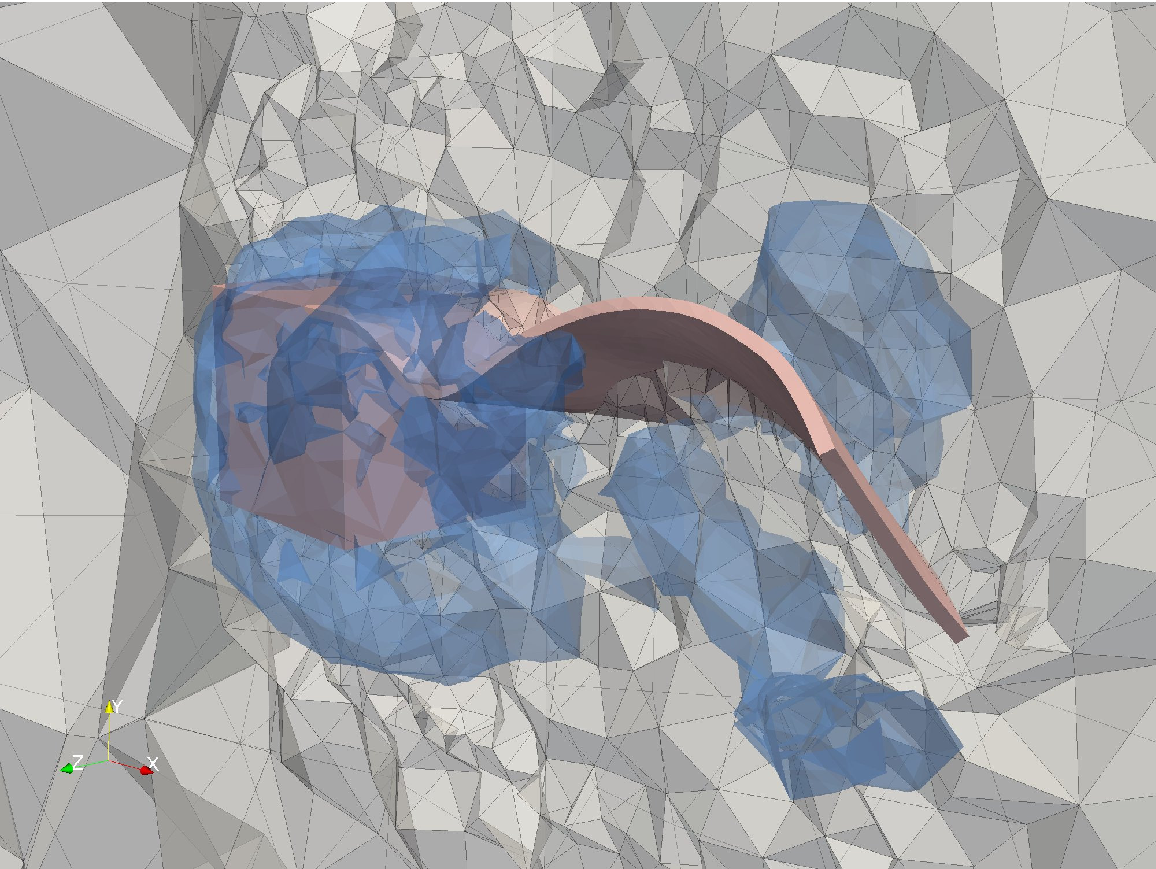
\includegraphics[width=\largefig]{chapters/hoffman-2/pdf/cube556.pdf}
  \caption{A fluid--structure interaction problem consisting of a flag
    mounted behind a cube in turbulent flow. The plot shows the
    fluid--structure interface, an isosurface of the pressure and a
    cut of the mesh.}
  \label{fig:flag3D}
\end{figure}

The Unicorn software is organized into three parts:
\begin{description}
\item[Library] The Unicorn library provides common solver technology
  such as automated time-stepping, error estimation, adaptivity, mesh
  smoothing and slip/friction boundary conditions.

\item[Solver] The Unicorn solver implements the G2 adaptive
  discretization method for the UC model by formulating the relevant
  weak forms. There are currently two primary solvers: incompressible
  fluids and solids (including fluid--structure interaction) and
  compressible Euler (only fluid). The long-term goal is a
  unification of the incompressible and compressible formulations.

\item[Applications] Associated to the solver(s) are applications such
  as computational experiments and benchmarks with certain geometries,
  coefficients and parameters. These are represented as stand-alone
  programs built on top of the Unicorn solver/library, running in
  either serial or parallel (currently restricted to incompressible
  flow).
\end{description}

\begin{figure}
  \centering
  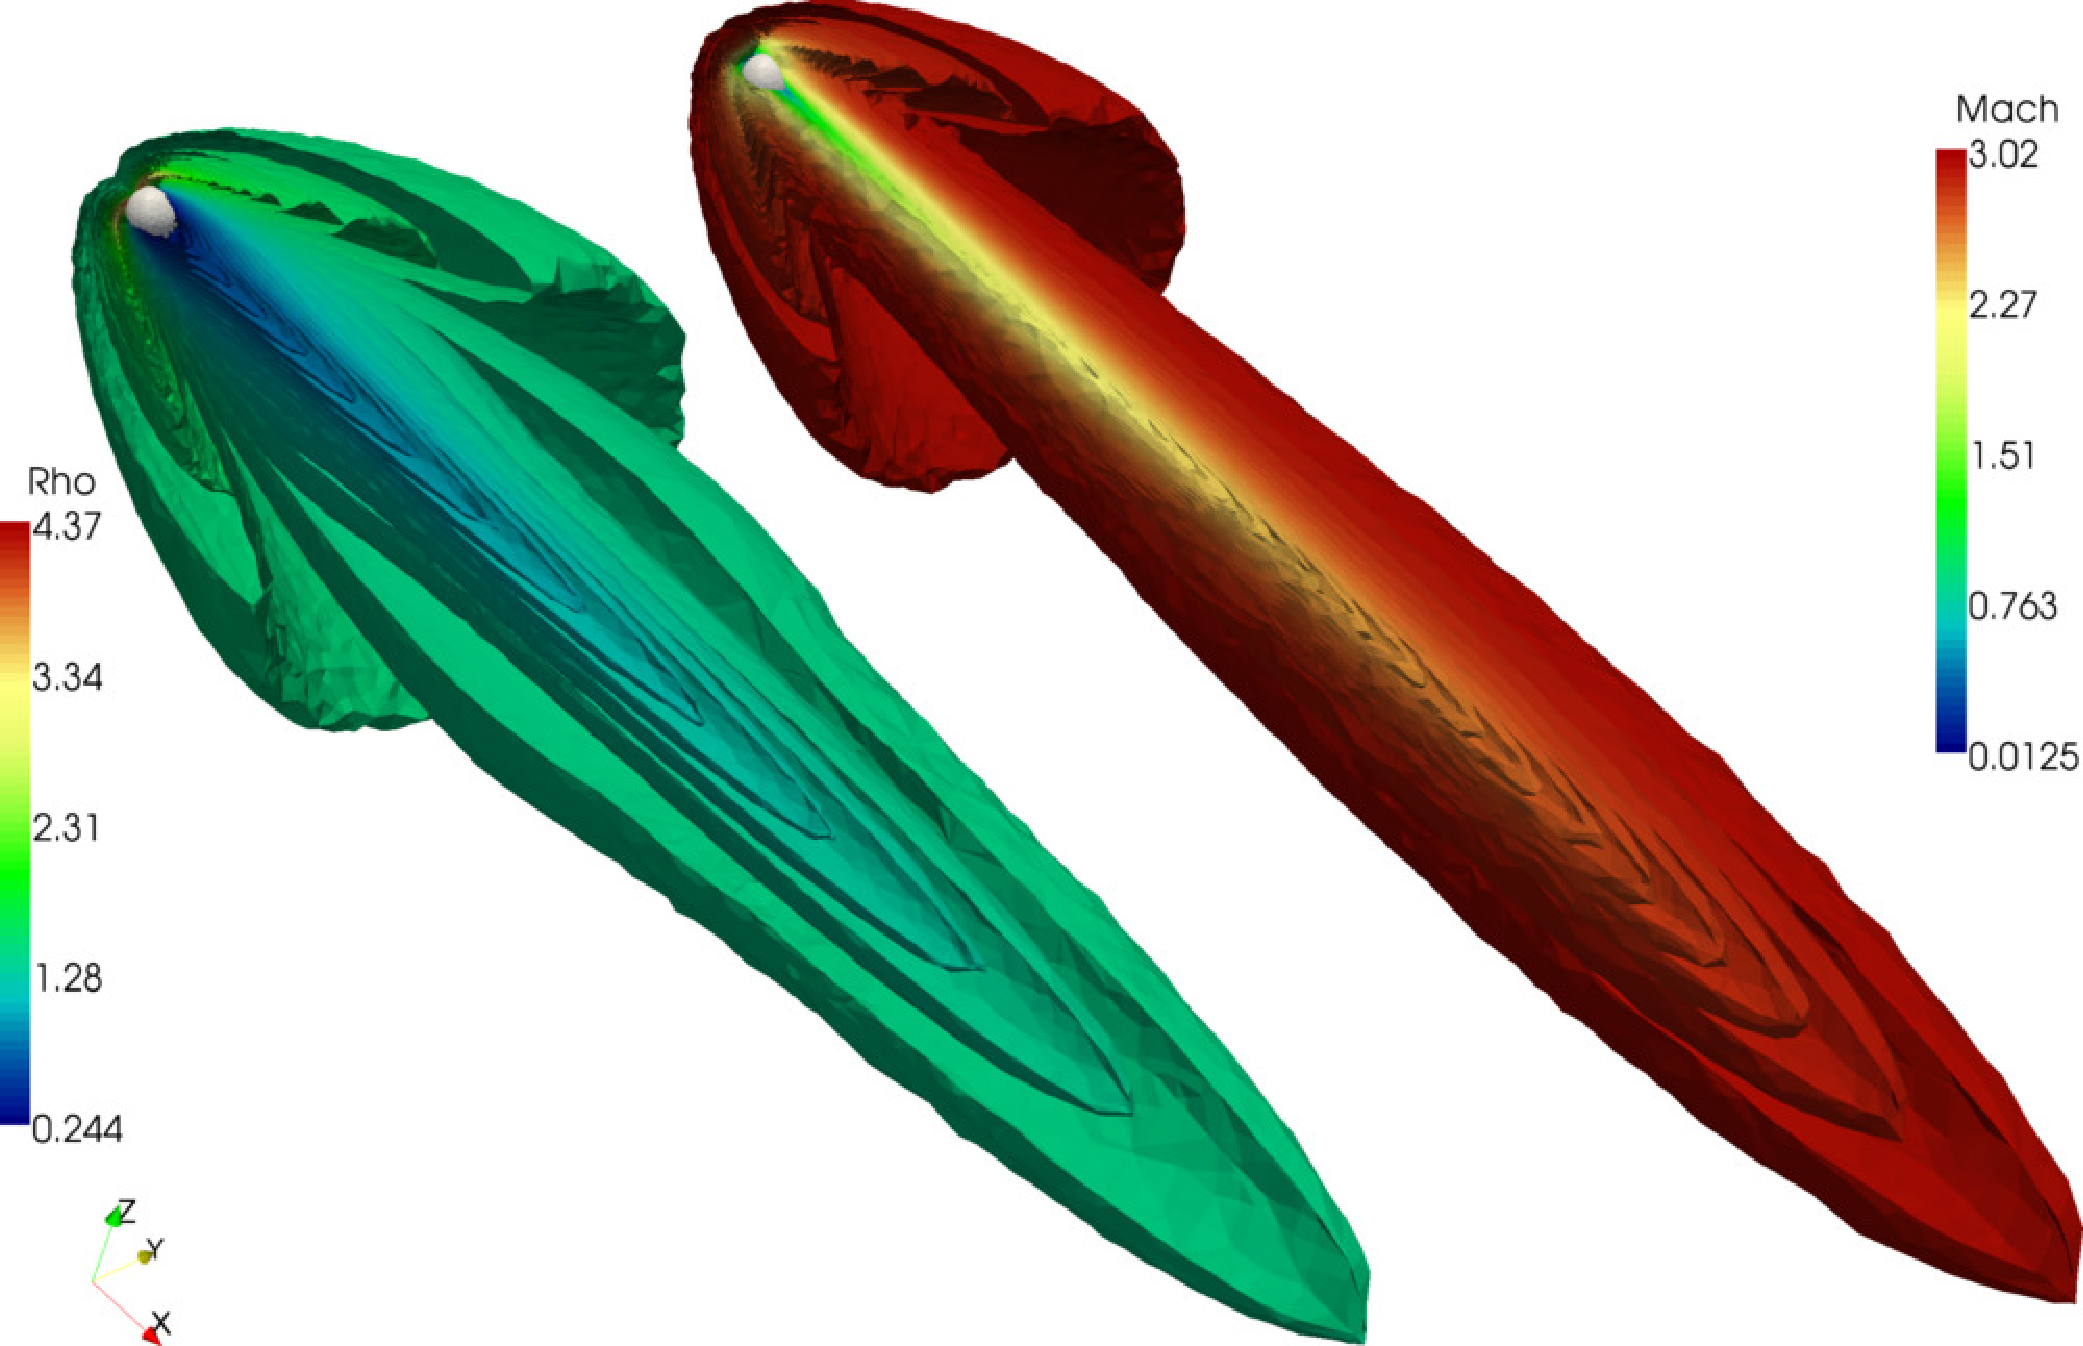
\includegraphics[width=\largefig]{chapters/hoffman-2/pdf/compressible3D.pdf}
  \caption{Example application of adaptive computation of 3D compressible
    flow around a sphere.}
  \label{fig:compr3D}
\end{figure}

\begin{figure}
  \centering
  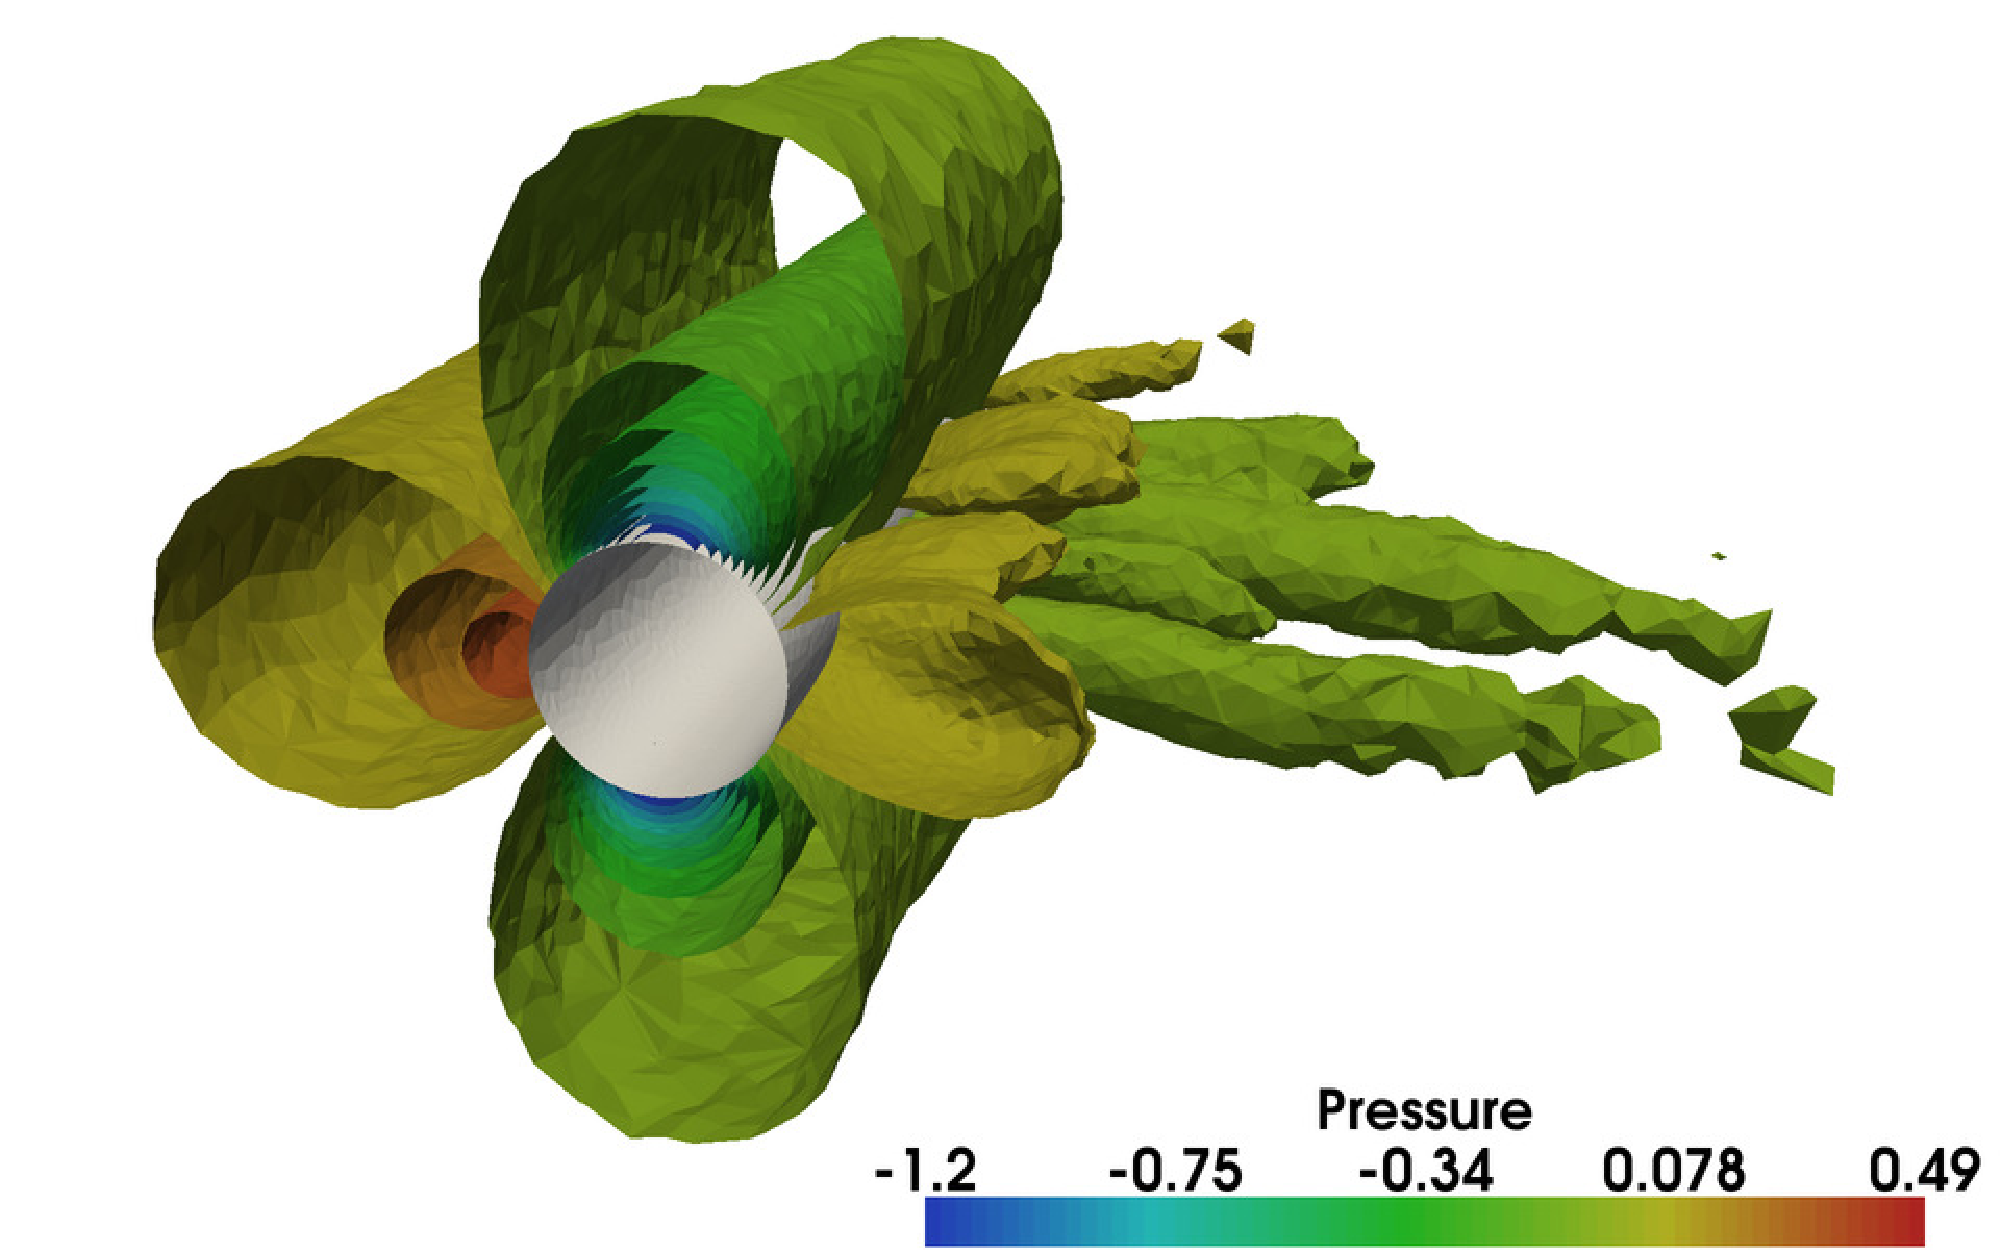
\includegraphics[width=\largefig]{chapters/hoffman-2/pdf/Hoffman_fig3d.pdf}
  \caption{Example application of 3D turbulent incompressible flow around
    a cylinder with parallel adaptive computation.}
  \label{fig:parcyl3D}
\end{figure}

\label{chapter:implementation:unicorn}

%------------------------------------------------------------------------------
\section{Unified continuum modeling}

We define, following classical continuum mechanics \citep{Gurtin1981},
a unified continuum model in a fixed Euler coordinate system
consisting of:
\begin{itemize}
\item conservation of mass,
\item conservation of momentum,
\item conservation of energy,
\item phase convection equation,
\item constitutive equations for stress as data,
\end{itemize}
where the stress is the Cauchy (laboratory) stress and the phase is an
indicator function used to determine which constitutive equation and
material parameters to use. Note that in this continuum description
the coordinate system is fixed (Euler), and a phase function
(indicator) is convected according to the phase convection
equation. The mesh is moved with the continuum velocity in the case of
a solid phase to eliminate diffusion of the phase interface. We
elaborate on this below in Section~\ref{sec:hoffman-2:ale}.

We define two variants of this model, incompressible and compressible,
where a future aim is to construct a unified
incompressible/compressible model and solver. We focus here the
presentation on the incompressible model.

We start with a model for conservation of mass and momentum, together
with a convection equation for a phase function $\theta$ over a
space-time domain $Q = \Omega \times [0, T]$ with $\Omega$ a bounded
open domain in $\mathbb{R}^3$ with boundary~$\Gamma$:
\begin{align}
    \frac{\partial \rho}{\partial t} + \frac{\partial}{\partial x_j} (u_j \rho) &= 0, \quad &\text{(mass conservation)}
\\
    \frac{\partial m_i}{\partial t} + \frac{\partial}{\partial x_j} (u_j m_i) &= \frac{\partial}{\partial x_j} \sigma_{ij} + f_i, \quad &\text{(momentum conservation)}
\\
    \frac{\partial \theta}{\partial t} + \frac{\partial}{\partial x_j} (u_j \theta) &= 0, \quad &\text{(phase convection equation)}
\end{align}
together with initial and boundary conditions, where $\rho$ is
density, $m_i = \rho u_i$ is momentum and $u_i$ is velocity.  If we
make the assumption that the continuum is incompressible; that is, $0
= D_t \rho = \frac{\partial}{\partial t} \rho + u_j
\frac{\partial}{\partial x_j} \rho$, it follows that we may express
the incompressible UC equations as
\begin{align}
  \rho\left(\frac{\partial u_i}{\partial t} + u_j \frac{\partial u_i}{\partial x_j} \right) &= \frac{\partial}{\partial x_j} \sigma_{ij} + f_i,
  \\
  \frac{\partial u_j}{\partial x_j} &= 0,
  \\
  \frac{\partial\theta}{\partial t} + u_j\frac{\partial\theta}{\partial x_j} &= 0.
\end{align}

We note that to model a fluid--structure interaction problem, we can
simply write the total stress $\sigma$ as a linear combination of
fluid and solid stress using the $\theta$ phase function: $\sigma = \theta \sigma_f + (1 - \theta) \sigma_s$.

The UC modeling framework is simple and compact, close to the
formulation of the original conservation equations, and does not
require mappings between different coordinate systems. This allows
simple manipulation and processing for error estimation and
implementation.

One key design choice of UC modeling is to define the Cauchy stress
$\sigma$ as data, which means the conservation equations are fixed
regardless of the choice of constitutive equation. This gives a
generality in method and software design, where a modification of the
constitutive equation impacts the formulation and implementation of
the constitutive equation, but not the formulation and implementation
of the conservation equations.

%------------------------------------------------------------------------------
\section{Space-time general Galerkin discretization}

Adaptive G2 methods (also referred to as Adaptive DNS/LES) have been
used in a number of turbulent flow computations to a very low
computational cost
\citep{Hoffman2005,HoffmanJohnson2006b,Hoffman2006,Hoffman2009,HoffmanJansson2009,VilelaJanssonEtAl2010},
where convergence is obtained in output quantities such as drag, lift
and pressure coefficients and Strouhal numbers, using orders of
magnitude fewer mesh points than with standard LES methods based on
\emph{ad~hoc} refined computational meshes.

\subsection{Standard Galerkin}

We begin by formulating the standard \cgone{}\cgone{} FEM
\citep{ErikssonEstepHansboEtAl1996} with piecewise continuous linear
solution in time and space for \eqref{eq:TotalModel}. We let $w = (u,
  p, \theta)$ denote the exact solution, $W = (U, P, \Theta)$ the
discrete solution, $v = (v^u, v^p, v^\theta)$ the test function and
$R(W) = (R_u(W), R_p(W), R_\theta(W))$ the residual. The residual is defined by
%%
\begin{equation} \label{eq:TotalModel}
  \begin{split}
    R_u(W) &= \rho\left(\frac{\partial U_i}{\partial t} + U_j \frac{\partial U_i}{\partial x_j} \right) - \frac{\partial}{\partial x_j} \Sigma_{ij} - f_i,\\
    R_p(W) &= \frac{\partial U_j}{\partial x_j},\\
    R_\theta(W) &= \frac{\partial\Theta}{\partial t} + U_j \frac{\partial \Theta}{\partial x_j},
  \end{split}
\end{equation}
%%
where $\Sigma$ denotes a discrete piecewise constant stress.

To compute the solution, we enforce the Galerkin orthogonality
\begin{equation}
  \inner{R(W)}{v} = 0
\end{equation}
for all functions $v$ in the test space $\hat{V}_{hk}$ consisting of
piecewise linear continuous functions in space and piecewise constant
discontinuous functions in time. Here $\inner{\cdot}{\cdot}$ denotes
the $L^2$-inner product in space and time.

This standard finite element formulation is unstable for
convection-dominated problems and also suffers from instabilities as a
result of equal order elements for the pressure and velocity. We
therefore add streamline--diffusion stabilization as described below.

The \cgone{}\cgone{} formulation with trapezoidal quadrature in time
is equivalent to Crank--Nicolson time-stepping with piecewise linear
elements in space. This has the advantage of being a very simple,
standard, and familiar discrete formulation.

\subsection{Local ALE}
\label{sec:hoffman-2:ale}

If the phase function $\Theta$ has different values on the same cell,
it would lead to an undesirable diffusion of the phase interface. By
introducing a moving space-time finite element space and mesh,
oriented along the characteristics of the convection of the phase
interface \citep[section concerning ``The characteristic Galerkin
  method'']{ErikssonEstepHansboEtAl1996}, we can define the phase
interface at cell facets, allowing the interface to stay
discontinuous.

We thus define a local ALE coordinate map as part of the
discretization on each space-time slab, where it is used to introduce
a mesh velocity. Note that we still compute with global Euler
coordinates, but with a moving mesh.

To be able to define and compensate for an arbitrary mesh velocity
$\beta_h$, we define a local coordinate map $\phi$ on each space-time
slab:
\begin{equation}
  \begin{split}\label{eq:ALEmap}
    \frac{\partial}{\partial t} \phi(t, \bar{x}) &= \beta_h(t, \bar{x}),
    \\
    (x, t) &= \phi(\bar{x}, t).
  \end{split}
\end{equation}
Application of the chain rule gives the relation
\begin{equation}
  \label{eq:ALE2}
  \frac{\partial}{\partial t} U(x,t) + U(x,t) \cdot \nabla U(x,t) = \frac{\partial}{\partial t} \bar{U}(\bar{x},t) +
  (\bar{U}(\bar{x},t) - \beta_h)) \cdot \nabla \bar{U}(\bar{x},t).
\end{equation}

Choosing $\beta_h = U$ in the solid part of the mesh gives a trivial
solution of the phase convection equation, and we can remove it from
the system. The resulting discrete UC equations are then defined by the residuals
\begin{equation}
  \begin{split}\label{eq:ALE}
    R_u(W) &= \rho\left(\frac{\partial U_i}{\partial t} + (U_j - \beta^h_j) \frac{\partial U_i}{\partial x_j} \right) - \frac{\partial}{\partial x_j} \Sigma_{ij} - f_i,
    \\
    R_p(W) &= \frac{\partial U_j}{\partial x_j}.
  \end{split}
\end{equation}

We thus choose the mesh velocity $\beta_h$ to be the discrete material
velocity $U$ in the structure part of the mesh (vertices touching
structure cells) and in the rest of the mesh we use mesh smoothing to
determine $\beta_h$ to maximize the mesh quality. Alternatively, one
may use local mesh modification operations (refinement, coarsening,
swapping) on the mesh to maintain the quality
\citep{Comp`ereRemacleJanssonEtAl2009}.

\subsection{Streamline--diffusion stabilization}

The standard FEM formulation is unstable.  We therefore consider a
weighted standard streamline--diffusion method of the form
$\inner{R(W)}{v + \delta R(v)} = 0$ for all $v \in \hat{V}_{hk}$ (see
\citet{ErikssonEstepHansboEtAl1996}) with $\delta > 0$ a stabilization
parameter. We make further simplifications by only including necessary
stabilization terms and dropping terms not contributing to
stabilization. Although not fully consistent, this avoids unnecessary
smearing of shear layers. For the UC model, the stabilized method thus
takes the following form:
%%
\begin{align}
  \inner{R^u(W)}{v^u} &=
  \inner{\rho(\frac{\partial U_i}{\partial t} + U_j \frac{\partial U_i}{\partial x_j} ) - f_i}{v^u_i} +
  \inner{\Sigma_{ij}}{\frac{\partial}{\partial x_j} v^u_i} + SD^u(W, v^u) = 0, \\
  \inner{R^p(W)}{v^p} &= \inner{\frac{\partial U_j}{\partial x_j}}{v^p} + SD^p(W, v^p) = 0,
\end{align}
for all $v \in \hat{V}_{hk}$, where
\begin{align}
  SD^u(W, v^u) &=
  \delta_1 \inner{U_j \frac{\partial U_i}{\partial x_j}}{U_j \frac{\partial v^u_i}{\partial x_j} } +
  \delta_2 \inner{\frac{\partial U_j}{\partial x_j}}{\frac{\partial v^u_j}{\partial x_j} }, \\
  SD^p(W, v^p) &= \delta_1 \inner{\frac{\partial P}{\partial x_i}}{\frac{\partial v^p}{\partial x_i}}.
\end{align}

%------------------------------------------------------------------------------
\section{Implementation}

We here present an overview of the design of Unicorn. The Unicorn
solver class \emp{UCSolver} ties together the technology in the
Unicorn library with other parts of FEniCS to expose an interface (see
listing \ref{code:UCSolver}) for simulating applications in continuum
mechanics. The main part of the solver implementation is the weak
forms for the G2 discretization of the UC model (see
Figure~\ref{code:FFC_UC}), together with forms for the stress and
residuals for the error estimation. Coefficients from the application
are connected to the form, and then time-stepping is carried out by
the class \emp{TimeDependentPDE}. Certain coefficients, such as the
$\delta$ stabilization coefficients are also computed as part of the
solver (not as forms). The solver computes one iteration of the
adaptive algorithm (primal solve, dual solve and mesh refinement),
where the adaptive loop is implemented by iteratively running the
solver for a sequence of meshes.

\begin{figure}
\begin{uflcode}
...

v = TestFunction(V)
U1 = TrialFunction(V) # Unknown velocity U
UP = TrialFunction(V) # U from previous iteration
U0 = Function(V)      # U from previous timestep
P = Function(VS)      # Pressure

UC = 0.5*(U0 + UP)

def epsilon(u):
    return sym(grad(u))

def S(u, P):
    return P*Identity(d) - nu*grad(u)

def f(u, v):
    return -inner(grad(u)*u, v) + \
        inner(S(u, P), grad(v)) + \
        -d1*inner(grad(u)*u, grad(v)*u) + \
        -d2*inner(div(u), div(v)) + \
        dot(fsource, v)

def dfdu(u, k, v):
    return -inner(grad(u)*UC, v) + \
        -inner(nu*grad(u), grad(v)) + \
        -d1*inner(grad(u)*UC, grad(v)*UC) + \
        -d2*inner(div(u), div(v))

# cG(1) in time
def F(u, u0, k, v):
    uc = 0.5 * (u + u0)
    return (-dot(u, v) + dot(u0, v) + k*f(u, v))

def dFdu(u, u0, k, v):
    uc = 0.5 * u
    return (-dot(u, v) + k*dfdu(uc, k, v))

a = (dFdu(U1, U0, k, v)) * dx
L = (dFdu(UP, U0, k, v) - F(UP, U0, k, v)) * dx
\end{uflcode}
\caption{Source code for the bilinear and linear forms for a Newton
  iteration (with approximate Jacobian) for solving the incompressible
  UC model.}
\label{code:FFC_UC}
\end{figure}

The \emp{UCSolver} implementation is parallelized for distributed
memory architectures using MPI, and we can show strong scaling for
hundreds of cores on several platforms (see
Figure~\ref{fig:hoffman-2:sp}). The entire adaptive algorithm is
parallel, including Rivara mesh refinement and \apriori{} predictive
load balancing. Unicorn can efficiently simulate massively parallel
applications for turbulent incompressible flow
\citep{JanssonHoffmanJansson2010, Jansson2011}. An example of a
parallel adaptive cylinder simulation is presented in
Figure~\ref{fig:parcyl3D}.

\begin{figure}
  \centering
  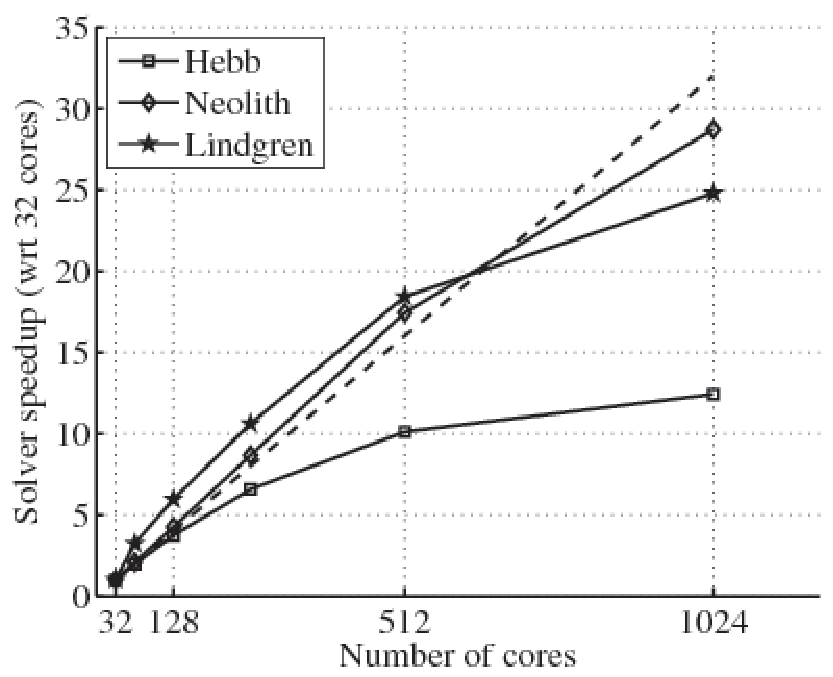
\includegraphics[width=\largefig]{chapters/hoffman-2/pdf/speedup_solve.pdf} \\
  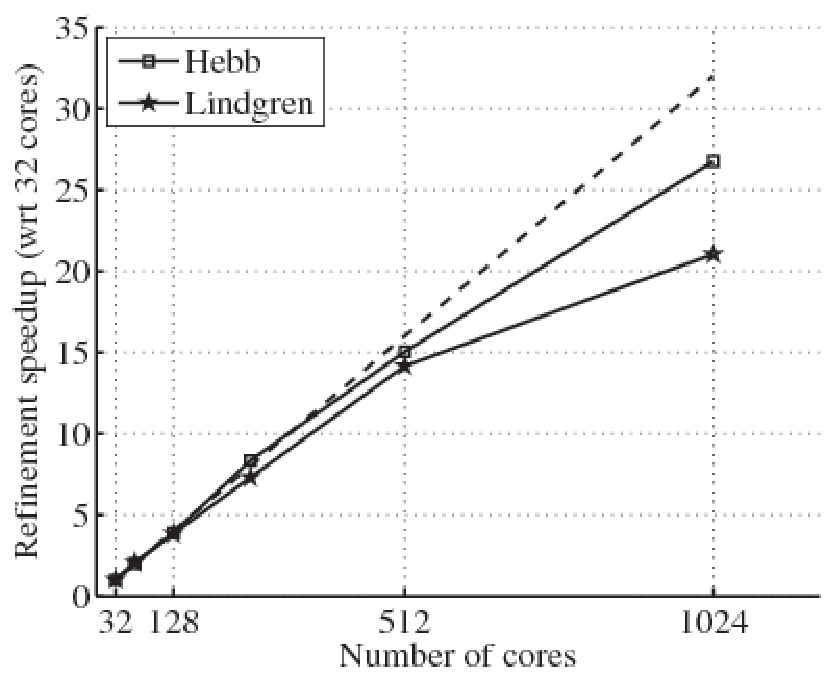
\includegraphics[width=\largefig]{chapters/hoffman-2/pdf/speedup_unrivara.pdf}
  \caption{\label{fig:hoffman-2:sp} Strong scaling results for mesh
    refinement and entire solver on several different architectures:
    \textit{Lindgren} (Cray XT6m), \textit{Hebb} (BlueGene/L) and
    \textit{Neolith} (regular Linux cluster with InfiniBand). The
    dashed lines refer to ideal speedup.}
\end{figure}

A compressible variant of the \emp{UCSolver} exists as the
\emp{CNSSolver} for adaptive G2 for compressible Euler flow. The
general method and algorithm is very close to that of the
\emp{UCSolver}, aside from the incompressibility. The long-term goal
is a unification of the incompressible/compressible formulations as
well. We refer to \citet{Nazarov2009} for implementation details of
the compressible \emp{CNSSolver}. See Figure~\ref{fig:compr3D} for an
example plot of compressible flow around a sphere.

\begin{figure}
\begin{c++}
class UCSolver :
  public TimeDependentPDE, public MeshAdaptInterface
{
public:
  /// Constructor: give boundary conditions,
  /// coefficients
  UCSolver(Function& U, Function& U0,
           Function** bisect, Mesh& mesh,
           Array <BoundaryCondition*>& bc_mom,
           Array <BoundaryCondition*>& bc_con,
           Function** f, real T, real nu,
           real mu, real rho_f, real rho_s,
           real u_bar, TimeDependent& t,
           PDEData* pdedata);

  /// Prescribe mesh size for MeshAdaptInterface
  virtual void updateSizeField();

  /// Allocate/deallocate PDE data for dynamic mesh
  /// adaptivity
  virtual void allocateAndComputeData();
  virtual void deallocateData();

  /// Compute mesh vertex coordinates and velocity
  void computeX();
  void computeW();

  /// Compute density, pressure, stress
  void computeRho();
  void computeP();
  void computeStress();

  /// Compute initial theta
  void computeTheta0();

  /// From TimeDependentPDE: time-stepping control
  void shift();
  bool update(real t, bool end);
  void preparestep();
  void prepareiteration();

  /// Assemble time step residual (L) right-hand
  /// side of Newton
  void rhs(const Vector& x, Vector& dotx, real T);

  /// Compute initial value
  void u0(Vector& x);

  /// Save solution/output quantities
  void save(Function& U, real t);

  /// Compute least-squares stabilization parameters
  /// (delta)
  void computeStabilization(Mesh& mesh, Function& w,
                            real nu, real k, real t,
                            Vector& d1vector,
                            Vector& d2vector);

  /// Deform/move mesh
  void deform(Mesh& mesh, Function& W, Function& W0);

  /// Smooth/optimize quality of all or part of the
  /// mesh
  void smoothMesh(bool bAdaptive);
}
\end{c++}
\caption{C++ class interface for the Unicorn class \emp{UCSolver}.}
\label{code:UCSolver}
\end{figure}

\subsection{Unicorn classes/interfaces}

Key concepts are abstracted in the following classes/interfaces:
%%
\begin{description}
\item[\emp{TimeDependentPDE}: \ time-stepping]
\ \\
In each time-step a nonlinear algebraic system is solved by
fixed-point iteration.
\item[\emp{ErrorEstimate}: \ adaptive error control] \ \\ Adaptivity
  is based on computing local {\em error indicators} of the
  form $\eta_K = \|h R(U)\|_T \|D Z\|_T$, where $Z$ is the so-called
  dual solution.

\item[\emp{SpaceTimeFunction}: \ space-time coefficient]
\ \\
Storage and evaluation of a space-time function/coefficient.
\item[\emp{SlipBC}: \ friction boundary condition] \ \\ Efficient
  computation of turbulent flow in Unicorn is based on modeling of
  turbulent boundary layers by a friction model, where the slip
  boundary condition $u \cdot n = 0$ is implemented strongly as part
  of the algebraic system.
\item[\emp{ElasticSmoother}: \ elastic mesh smoothing/optimization]
\ \\
Optimization of cell quality according to an elastic analogy.
\item[\emp{MeshAdaptInterface}: \ mesh adaptation interface]
\ \\
Abstraction of the interface to the MAdLib package for mesh adaptation
using local mesh operations.
\end{description}

\subsection{\emp{TimeDependentPDE}}

We consider general time-dependent equations of the type
$\frac{\partial}{\partial t} u + A(u) = 0$, where $A$ denotes a
possibly nonlinear differential operator in space. We want to define a
class (data structures and algorithms) abstracting the time-stepping
of the G2 method. The equation is given as input and the time-stepping
should be generated automatically. We do this for the \cgone{}\cgone{}
method by applying a simplified Newton's method. This is encapsulated
in a C++ class interface in
Figure~\ref{code:TimeDependentPDE} called \emp{TimeDependentPDE}.

\begin{figure}
\begin{c++}
/// Represent and solve time dependent PDE.
class TimeDependentPDE
{
  /// Public interface
public:
  TimeDependentPDE(
   // Computational mesh
   Mesh& mesh,
   // Bilinear form for Jacobian approx.
   Form& a,
   // Linear form for time-step residual
   Form& L,
   // List of boundary conditions
   Array <BoundaryCondition*>& bcs,
   // End time
   real T);

  /// Solve PDE
  virtual uint solve();

protected:
  /// Compute initial value
  virtual void u0(Vector& u);
  /// Called before each time step
  virtual void preparestep();
  /// Called before each fixed-point iteration
  virtual void prepareiteration();
  /// Return the bilinear form a
  Form& a();
  /// Return the linear form L
  Form& L();
  /// Return the mesh
  Mesh& mesh();
};
\end{c++}
\caption{C++ class interface for \emp{TimeDependentPDE}.}
\label{code:TimeDependentPDE}
\end{figure}
The skeleton of the time-stepping with fixed-point iteration is
implemented in listing \ref{code:time-stepping}.

\begin{figure}
\begin{c++}
void TimeDependentPDE::solve()
{
  // Time-stepping
  while (t < T)
  {
    U = U0;
    preparestep();
    step();
  }
}

void TimeDependentPDE::step()
{
  // Fixed-point iteration
  for(int iter = 0; iter < maxiter; iter++)
  {
    prepareiteration();
    step_residual = iter();

    if (step_residual < tol)
    {
      // Iteration converged
      break;
    }
  }
}

void TimeDependentPDE::iter()
{
  // Compute one fixed-point iteration
  assemble(J, a());
  assemble(b, L());
  for (uint i = 0; i < bc().size(); i++)
    bc()[i]->apply(J, b, a());
  solve(J, x, b);

  // Compute residual for the time-step/fixed-point
  // equation
  J.mult(x, residual);
  residual -= b;

  return residual.norm(linf);
}
\end{c++}
\caption{Skeleton implementation in Unicorn of time-stepping with
fixed-point iteration.}
\label{code:time-stepping}
\end{figure}

We use a block-diagonal quasi-Newton method, where we start by
formulating the full Newton method and then drop terms off the
diagonal blocks. We also use the constitutive law as an identity to
express $\Sigma$ in terms of $U$, allowing larger time steps than
would be possibly otherwise by iterating between $\Sigma$ and $U$.
See \citet{Jansson2009} for a discussion about the efficiency of the
fixed-point iteration and its implementation.

\subsection{\emp{ErrorEstimate}}

The duality-based adaptive error control algorithm requires the
following components:

\begin{description}
\item[Residual computation] We compute the mean-value in each cell of
  the residual $R(U)$ by an $L^2$-projection into the space of piecewise
  constants.
\item[Dual solution] We compute the solution of the dual problem using
  the same technology as the primal problem. The dual problem is
  solved backward in time, but using the time coordinate transform $s =
  T - t$ we can use the standard \emp{TimeDependentPDE} interface.
\item[Space-time function storage/evaluation] We compute error
  indicators while solving the dual problem as space-time integrals
  over cells: $\eta_T = \inner{R(U)}{\frac{\partial}{\partial x} Z}$, where
  we need to evaluate both the primal solution $U$ and the dual
  solution $Z$. In addition, $U$ is a coefficient in the dual
  equation. This requires storage and evaluation of a space-time
  function, which is encapsulated in the \emp{SpaceTimeFunction}
  class.
\item[Mesh adaptation] After the computation of the error indicators,
  we select the largest $p\%$ of the indicators for refinement. The
  refinement is then performed by recursive Rivara cell bisection.
  Alternatively, one may use MAdLib
  \citep{Comp`ereRemacleJanssonEtAl2009} for more general mesh
  adaptation based on edge split, collapse and swap operations.
\end{description}

Using these components, we can construct an adaptive algorithm. The
adaptive algorithm is encapsulated in the C++ class interface in
Figure~\ref{code:ErrorEstimate} which we call \emp{ErrorEstimate}.

\begin{figure}
\begin{c++}
/// Estimate error as local error indicators based
/// on duality
class ErrorEstimate
{
public:

  /// Constructor (give components of UC residual
  /// and dual solution)
  ErrorEstimate(Mesh& mesh,
		Form* Lres_1,
		Form* Lres_2,
		Form* Lres_3,
		Form* LDphi_1,
		Form* LDphi_2,
		Form* LDphi_3);

  // Compute error (norm estimate)
  void ComputeError(real& error);

  // Compute error indicator
  void ComputeErrorIndicator(real t, real k,
                             real T);

  // Compute largest indicators
  void ComputeLargestIndicators(
    std::vector<int>& cells,
    real percentage);

  // Refine based on indicators
  void AdaptiveRefinement(real percentage);
}
\end{c++}
\caption{C++ class interface for \emp{ErrorEstimate}.}
\label{code:ErrorEstimate}
\end{figure}

\subsection{\emp{SpaceTimeFunction}}

The error estimation algorithm requires, as part of solving the dual
problem, the evaluation of space-time coefficients appearing in the
definition of the dual problem. In particular, we must evaluate the
primal solution $U$ at time $s = T - t$.  This requires storage and
evaluation of a space-time function, which is encapsulated in the
\emp{SpaceTimeFunction} class (see listing
\ref{code:SpaceTimeFunction}).

The space-time functionality is implemented as a list of space
functions at regular sample times, where evaluation is piecewise
linear interpolation in time of the degrees of freedom.

\begin{figure}
\begin{c++}
/// Representation of space-time function (storage
/// and evaluation)
class SpaceTimeFunction
{
public:

  /// Create space-time function
  SpaceTimeFunction(Mesh& mesh, Function& Ut);

  /// Evaluate function at time t, giving result in
  /// Ut
  void eval(real t);

  // Add a space function at time t
  void addPoint(std::string Uname, real t);

  /// Return mesh associated with function
  Mesh& mesh();

  /// Return interpolant function
  Function& evaluant();
}
\end{c++}
\caption{C++ class interface for \emp{SpaceTimeFunction}.}
\label{code:SpaceTimeFunction}
\end{figure}

\subsection{\emp{SlipBC}}

For high Reynolds number problems such as car aerodynamics or airplane
flight, it is not possible to resolve the turbulent boundary
layer. One possibility is then to model turbulent boundary layers by a
friction model:
%%
\begin{align}
u \cdot n &= 0,
\\
\beta u \cdot \tau_k + (\sigma n) \cdot \tau_k &= 0, k = 1, 2.
\end{align}
%%
We implement the normal component condition (slip) boundary condition
strongly. By ``strongly'' we here mean an implementation of the
boundary condition after assembling the left-hand side matrix and the
right-hand side vector in the algebraic system, whereas the tangential
components (friction) are implemented ``weakly'' by adding boundary
integrals in the variational formulation. The row of the matrix and
load vector corresponding to a degree of freedom is found and replaced
by a new row according to the boundary condition.

The idea is as follows: Initially, the test function $v$ is expressed
in the Cartesian standard basis $(e_1, e_2, e_3)$.  Now, the test
function is mapped locally to normal-tangent coordinates with the
basis $(n, \tau_1, \tau_2)$, where $n = (n_1, n_2, n_3)$ is the
normal, and $\tau_1 = (\tau_{11}, \tau_{12}, \tau_{13})$, $\tau_2 =
(\tau_{21}, \tau_{22}, \tau_{23})$ are tangents to each node on the
boundary. This allows us to let the normal direction be constrained
and the tangent directions be free:
\begin{equation}
  v = (v \cdot n)n + (v \cdot \tau_1) \tau_1 + (v \cdot \tau_2) \tau_2.
\end{equation}
For the matrix and vector this means that the rows corresponding to the
boundary need to be multiplied with $n,\tau_1,\tau_2$, respectively,
and then the normal component of the velocity should be set to zero.

This concept is encapsulated in the class \emp{SlipBC} which is a
subclass of \emp{dolfin::BoundaryCondition} for representing strong
boundary conditions. For more details about the implementation of slip
boundary conditions,we refer to \citet{Nazarov2009}.

\subsection{\emp{ElasticSmoother}}

\begin{figure}
\begin{python}
V = VectorFunctionSpace(mesh, "Lagrange", 1)
VT = TensorFunctionSpace(mesh, "Lagrange", 1)

v = TestFunction(VV)
F = Function(VV)
U = Function(V)

def f(U, F, v):
    return -inner(F*grad(U), v) - inner(grad(U).T*F, v)

# icv is inverse cell volume
L = (icv*(dot(F0m, vm) + k*f(U, Fm, vm)))*dx
\end{python}
\caption{Source code for the form representing one time step for the
deformation gradient (F) evolution in the elastic smoother variant of
the UC model.}
\label{code:FFC_ElasticSmoother}
\end{figure}

\begin{figure}
  \center
  \begin{tabular}{cc}
    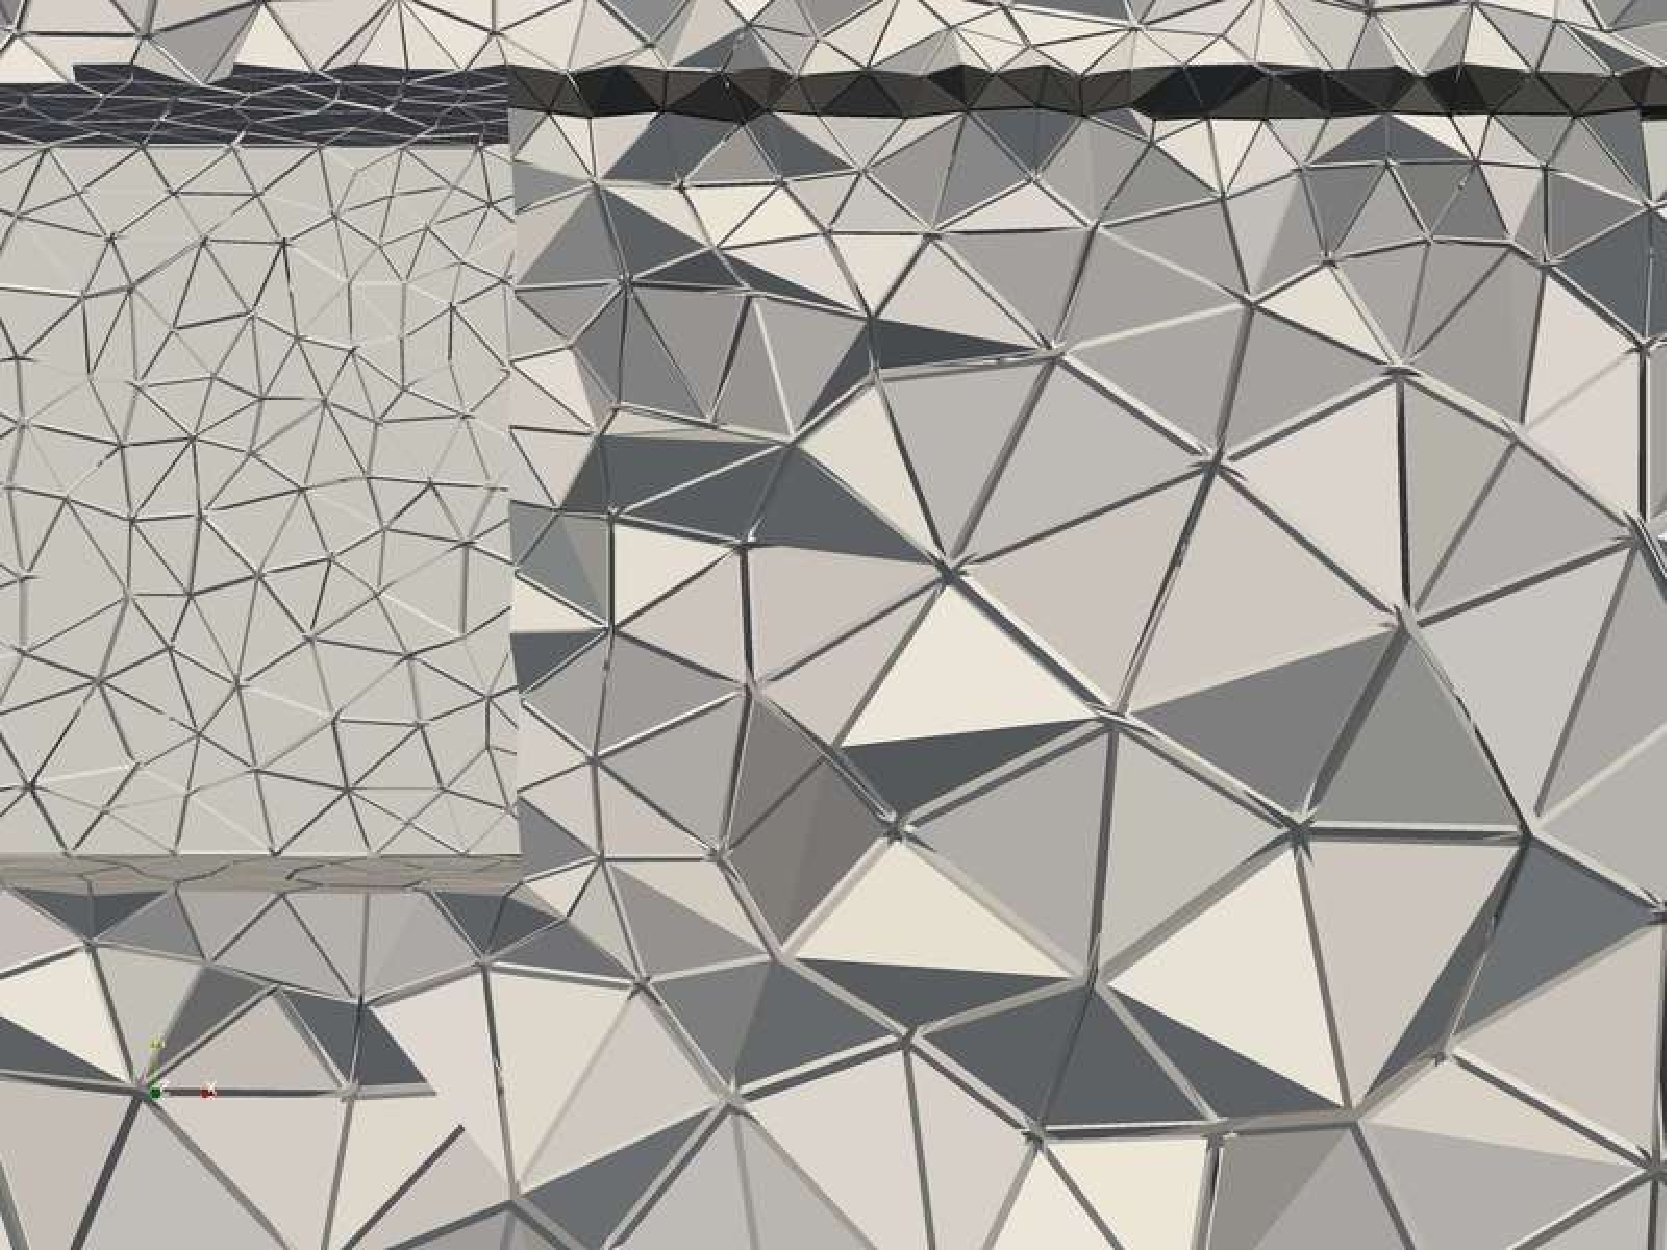
\includegraphics[width=\twofigs]{chapters/hoffman-2/pdf/force_smooth01.pdf} &
    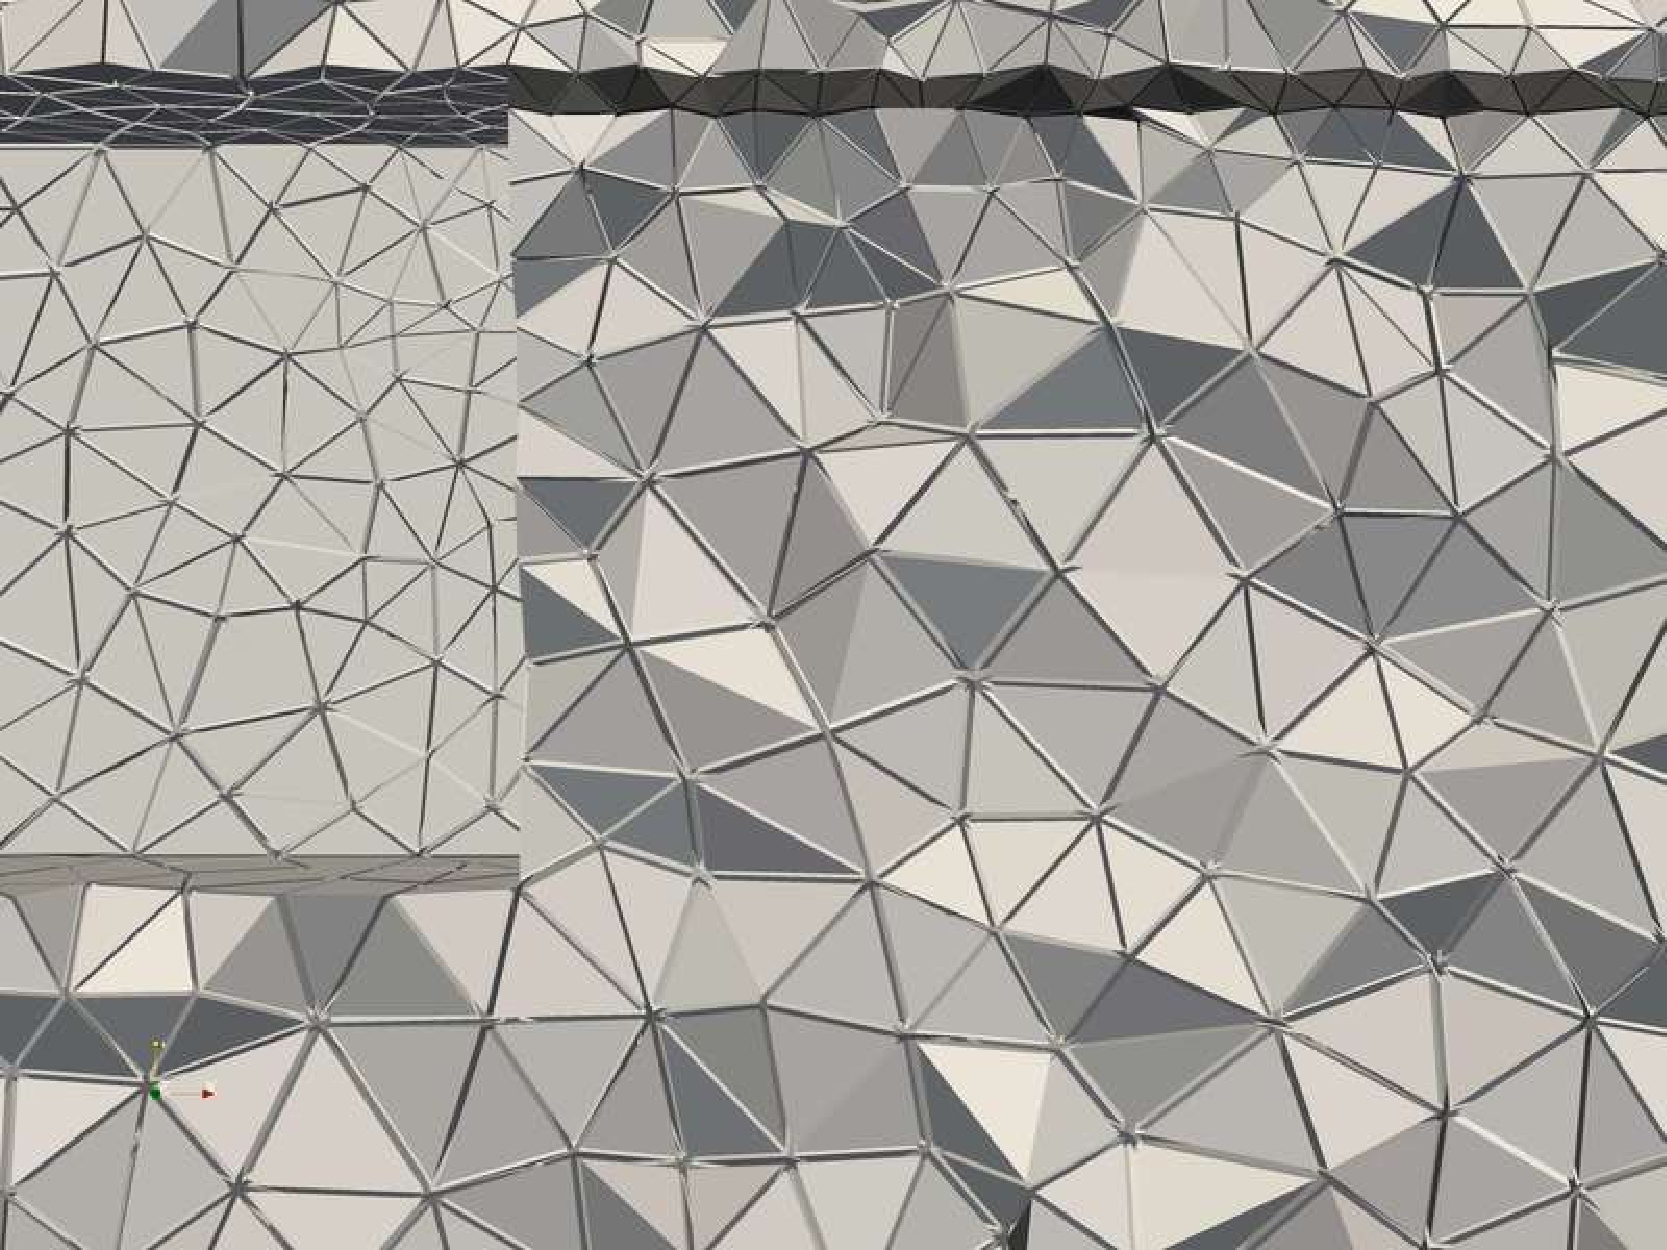
\includegraphics[width=\twofigs]{chapters/hoffman-2/pdf/force_hybrid01.pdf}\\
    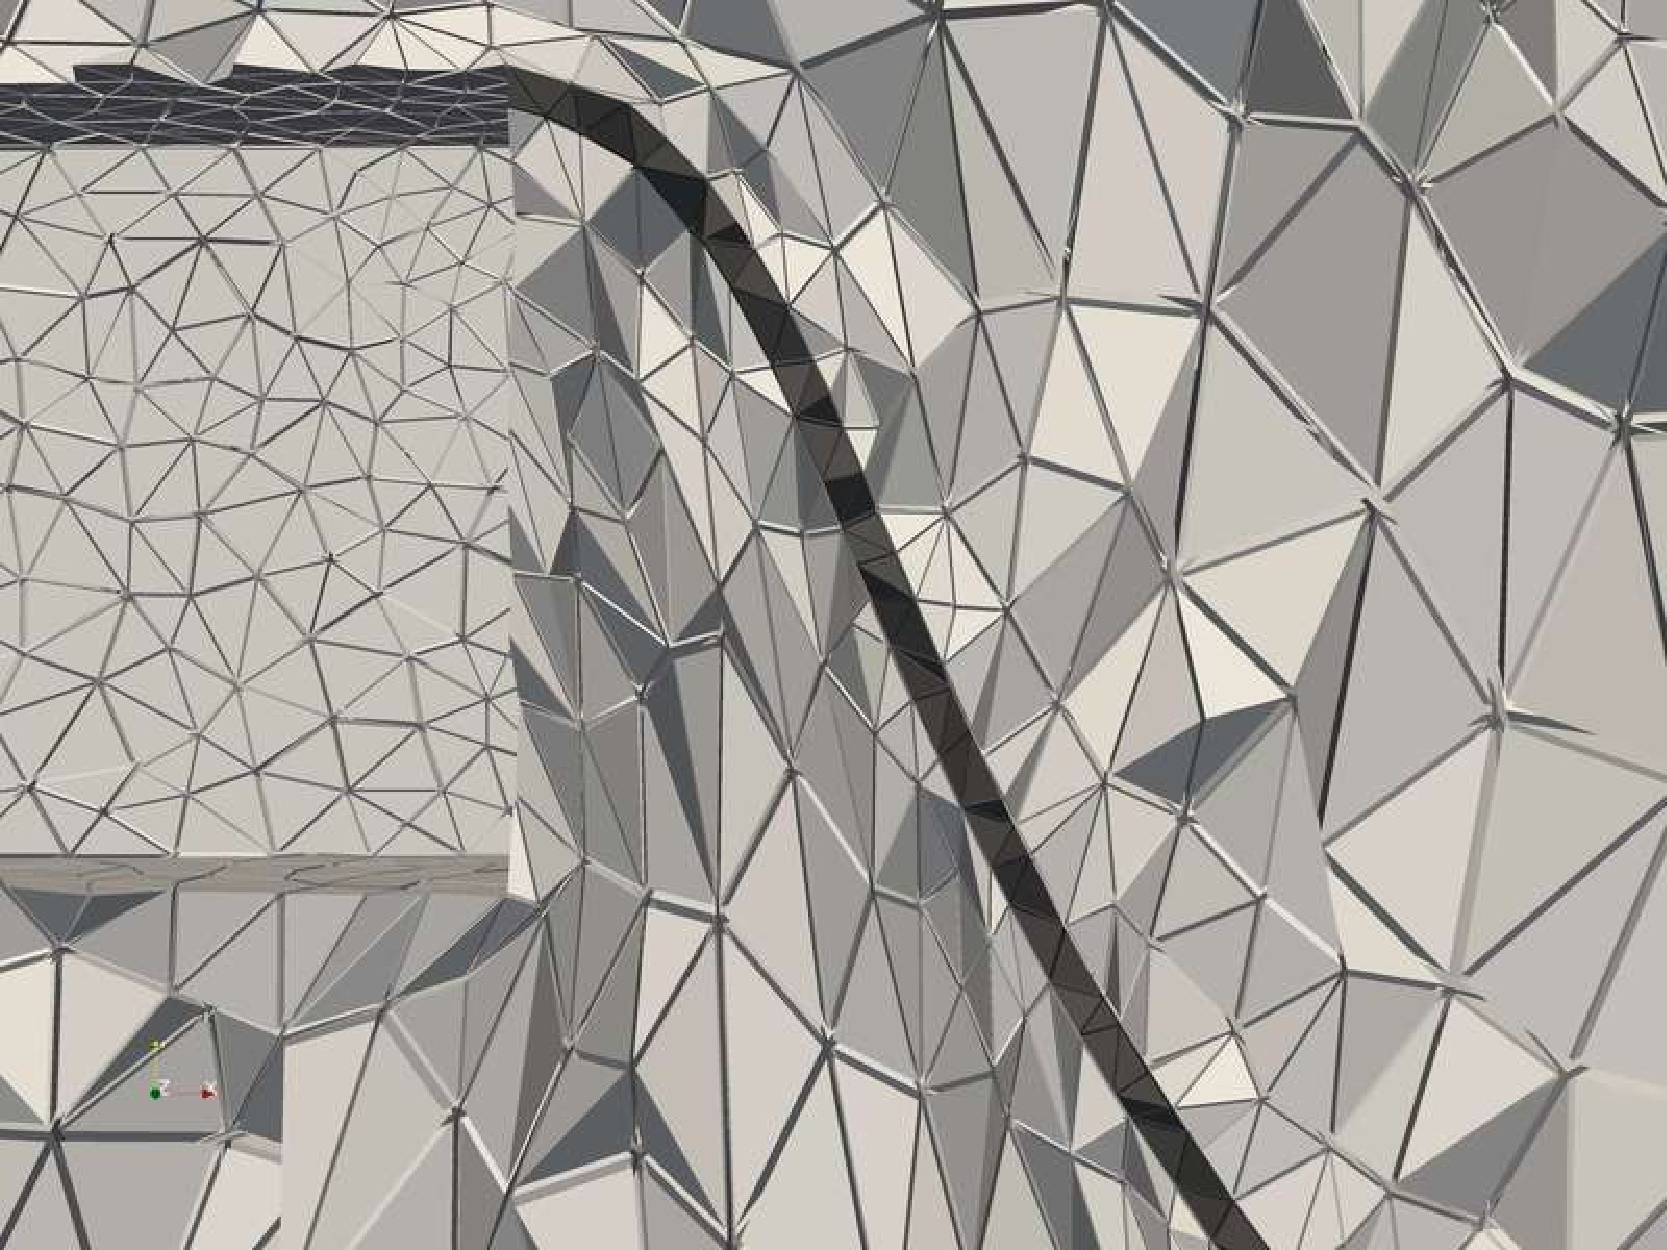
\includegraphics[width=\twofigs]{chapters/hoffman-2/pdf/force_smooth02.pdf} &
    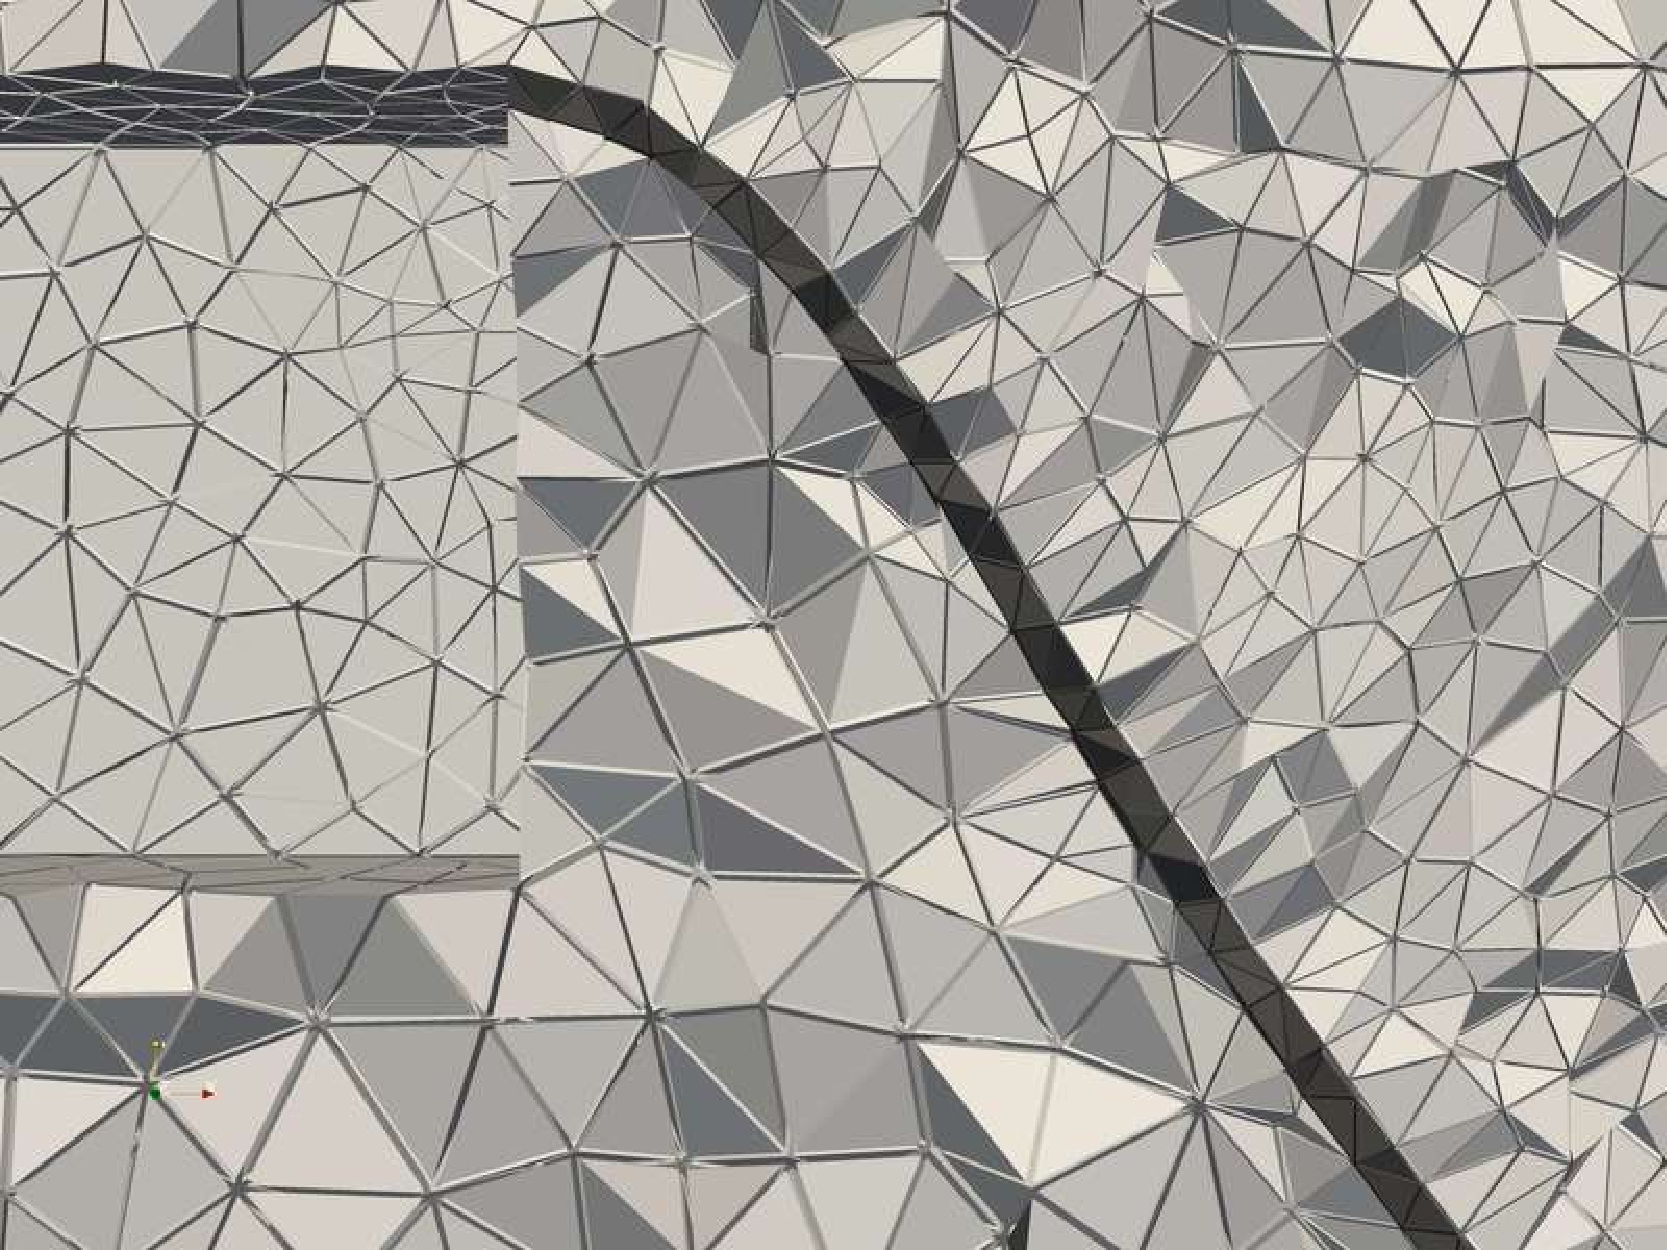
\includegraphics[width=\twofigs]{chapters/hoffman-2/pdf/force_hybrid02.pdf}\\
    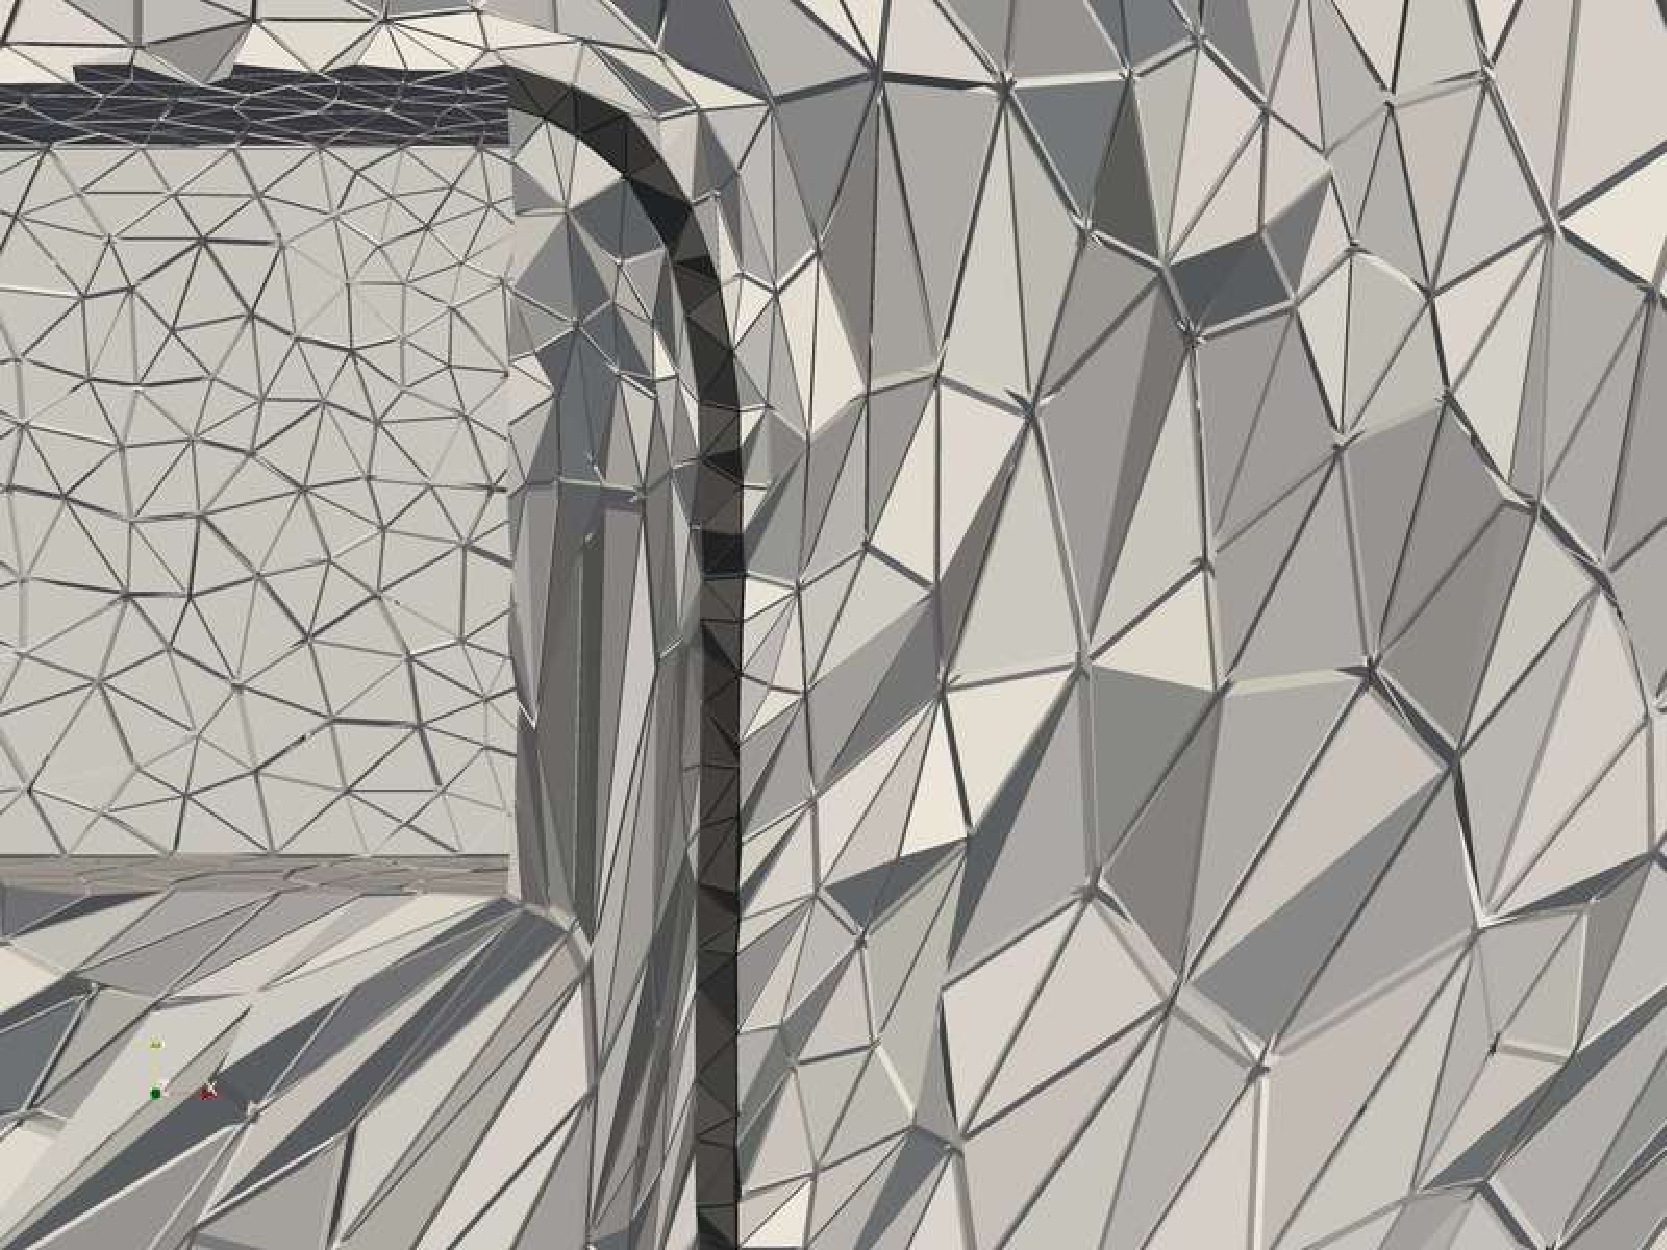
\includegraphics[width=\twofigs]{chapters/hoffman-2/pdf/force_smooth03.pdf} &
    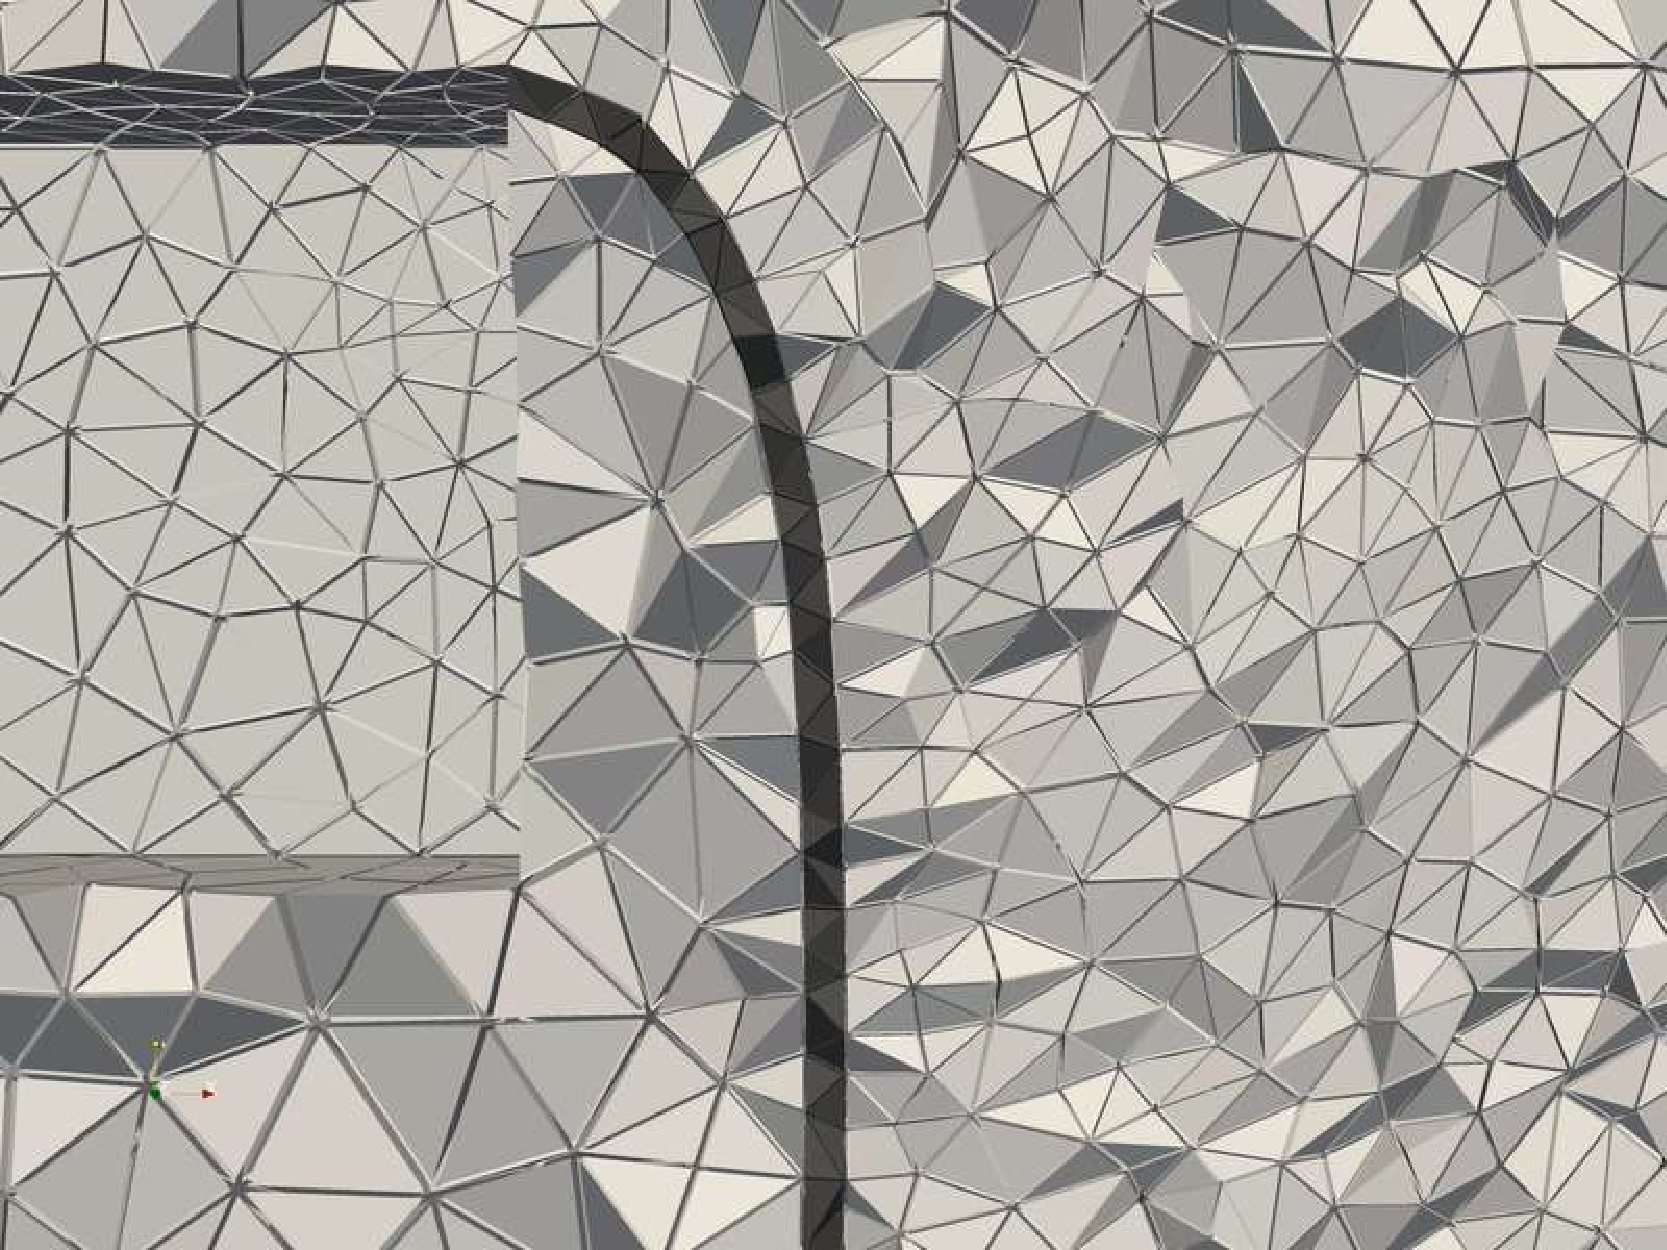
\includegraphics[width=\twofigs]{chapters/hoffman-2/pdf/force_hybrid03.pdf}\\
    (a) & (b)
  \end{tabular}
  \caption{Robustness test with (a) elastic smoothing and (b) mesh
    adaptation. Note the badly shaped cells squeezed between the cube
    and flag.}
  \label{fig:flag_robustness}
\end{figure}

\begin{figure}
\begin{c++}
/// Optimize cell quality according to elastic
/// variant of UC model
class ElasticSmoother
{
public:

  ElasticSmoother(Mesh& mesh);

  /// Smooth smoothed_cells giving mesh velocity W
  /// over time step k with h0 the prescribed cell
  /// size
  void smooth(MeshFunction<bool>& smoothed_cells,
              MeshFunction<bool>& masked_cells,
              MeshFunction<real>& h0,
              Function& W, real k);

  /// Extract submesh (for smoothing only marked cells)
  static void
  submesh(Mesh& mesh, Mesh& sub,
	  MeshFunction<bool>& smoothed_cells,
	  MeshFunction<int>& old2new_vertex,
	  MeshFunction<int>& old2new_cell);

}
\end{c++}
\caption{C++ class interface for {\emp{ElasticSmoother}}.}
\label{code:ElasticSmoother}
\end{figure}

To maintain a discontinuous phase interface in the UC model, we define
the mesh velocity $\beta_h$ as the discrete velocity $U$ in the solid
phase (specifically on the interface). The mesh velocity in the fluid
can be chosen more arbitrarily, but has to satisfy mesh quality and
size criteria. We construct a cell quality optimization/smoothing
method based on a pure elastic variant of the UC (see the form in
Figure~\ref{code:FFC_ElasticSmoother}). We define the following
requirements for the mesh velocity~$\beta_h$:
%%
\begin{enumerate}
\item $\beta_h = U$ in the solid phase part of the mesh.
\item Bounded mesh quality $Q$ defined by $$Q = \frac{d \| F
  \|_F^2}{\det(F)^{\frac{2}{d}}},$$ where $d$ is the spatial dimension, in
  the fluid part of the mesh. Preferably the mesh smoothing should
  improve $Q$ if possible.
\item Maintain mesh size $h(x)$ close to a desired $\hat{h}(x)$ given
  by \apost{} error estimation in an adaptive algorithm.
\end{enumerate}
%%
Mesh smoothing is handled in Unicorn by an elastic model using the
constitutive law $\sigma = \mu(I - (FF^\top)^{-1})$ where we recall
$F$ as the deformation gradient. We use the update law:
$\frac{\partial}{\partial t} F^{-1} = -F^{-1} \nabla u$ where we thus
need an initial condition for $F$. We set the initial condition $F_0 =
\bar{F}$ where $\bar{F}$ is the deformation gradient with regard to a
scaled equilateral reference cell, representing the optimal shape with
quality~$Q = 1$.

Solving the elastic model can thus be seen as optimizing for the
highest global quality $Q$ in the mesh. We also introduce a weight on
the Young's modulus $\mu$ for cells with low quality, penalizing high
average, but low local quality over mediocre global quality. We refer
to the source code for more details.

Unicorn provides the \emp{ElasticSmoother} class (see listing
\ref{code:ElasticSmoother}, which can be used to smooth/optimize for
quality in all or part of the mesh.

We perform a robustness test of the elastic smoothing and the mesh
adaptivity shown in \ref{fig:flag_robustness} where we use the same
geometry as the turbulent 3D flag problem, but define a zero inflow
velocity and instead add a gravity body force to the flag to create a
very large deformation with the flag pointing straight down. Both the
elastic smoothing and the mesh adaptivity compute solutions, but as
expected, the elastic mesh smoothing eventually cannot control the
cell quality; there does not exist a mesh motion which can handle
large rigid body rotations while bounding the cell quality.

\subsection{\emp{MeshAdaptInterface}}

A critical component in the adaptive algorithm as described above is
{\em mesh adaptivity}, which we define as constructing a mesh
satisfying a given mesh size function~$h(x)$.

We start by presenting the Rivara recursive bisection algorithm
\citep{Rivara1992} as a basic choice for mesh adaptivity (currently
the only available choice for parallel mesh adaptivity), but which can
only refine and not coarsen. Then the more general MAdLib is
presented, which enables full mesh adaptation to the prescribed
$h(x)$ through local mesh operations: edge split, edge collapse and
edge swap.

\paragraph{Rivara recursive bisection}

The Rivara algorithm bisects (splits) the longest edge of a cell, thus
replacing the cell with two new cells, and uses recursive bisection to
eliminate non-conforming cells with hanging nodes.
%%
\begin{algorithm}
\caption{The Rivara recursive bisection algorithm}
\label{alg:rivara}
\begin{algorithmic}
\Procedure{bisect}{$T$}
\State Split longest edge $e$
\While{$T_i(e)$ is non-conforming}
\State BISECT($T_i$)
\EndWhile
\EndProcedure
\end{algorithmic}
\end{algorithm}
%%
The same algorithm holds in both 2D/3D (triangles/tetrahedra). In 2D,
it can be shown \citep{Rivara1992} that the algorithm terminates in a
finite number of steps, and that the minimum angle of the refined mesh
is at least half the minimum angle of the starting mesh. In practice,
the algorithm produces excellent quality refined meshes both in 2D and
3D.

\paragraph{Local mesh operations: MAdLib}

\begin{figure}
  \centering
  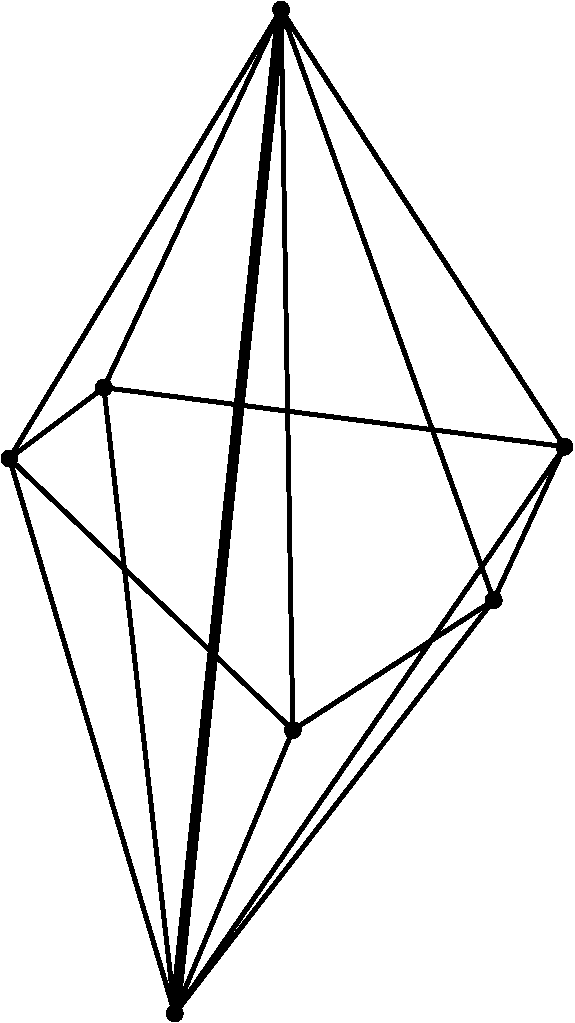
\includegraphics[width=\largefig]{chapters/hoffman-2/pdf/swap.pdf} \\
  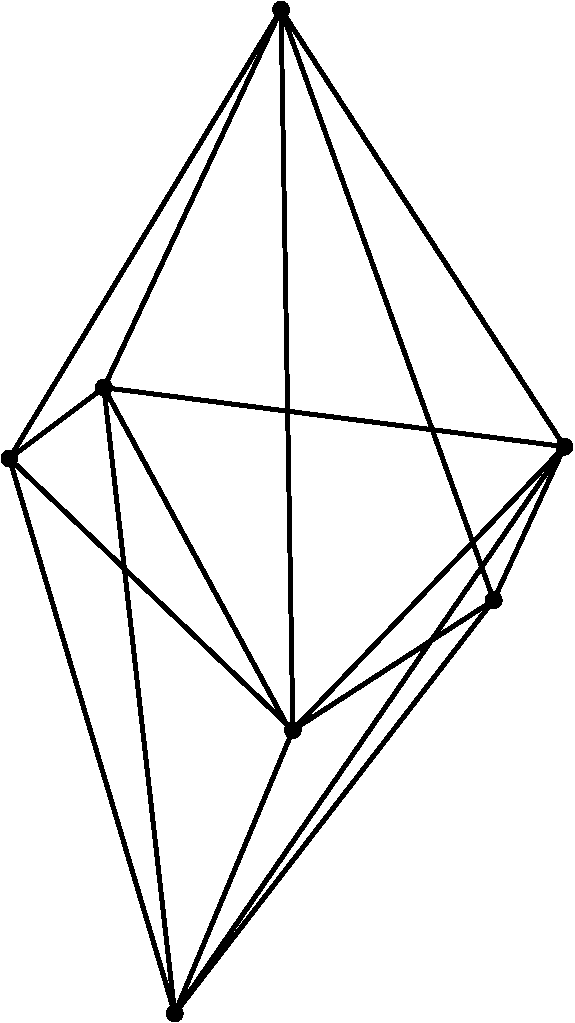
\includegraphics[width=\largefig]{chapters/hoffman-2/pdf/swap_config1.pdf}
  \caption{Edge swap operation: (top) initial cavity with swap edge
  highlighted and (bottom) possible configuration after the swap.}
\label{fig:op:eswap}
\end{figure}

MAdLib incorporates an algorithm and implementation of mesh adaptation
in which a small set of local mesh modification operators are defined
such as edge split, edge collapse and edge swap (see
Figure~\ref{fig:op:eswap} for an illustration of the edge swap
operator). A mesh adaptation algorithm is defined which uses this set
of local operators in a control loop to satisfy a prescribed size
field $h(x)$ and quality tolerance. Edge swapping is the key operator
for improving the quality of cells, for example around a vertex with a
large number of connected edges.

In the formulation of finite element methods, it is typically assumed
that the cell size of a computational mesh can be freely modified to
satisfy a desired size field $h(x)$ or to allow mesh motion. In
state-of-the-art finite element software implementations, this is
seldom the case \citep{BangerthHartmannKanschat2007, COMSOL2009}.

The mesh adaptation algorithm in MAdLib gives the freedom to adapt to
a specified size field using local mesh operations. The implementation
is published as free/open-source software.

Unicorn provides the \emp{MeshAdaptInterface} class (see listing
\ref{code:MeshAdaptInterface}), where one can subclass and implement
virtual functions to control the mesh adaptation using MAdLib.

\begin{figure}
\begin{c++}
/// Interface to MAdLib for mesh adaptation using
/// local operations Subclass and implement the
/// virtual functions
class MeshAdaptInterface
{
public:
  MeshAdaptInterface(Mesh *);

protected:
  /// Start mesh adaptation algorithm
  void adaptMesh();

  /// Give cell size field
  virtual void updateSizeField() = 0;

  /// Allocate and deallocate solver data
  virtual void deallocateData() = 0;
  virtual void allocateAndComputeData() = 0;

  /// Constrain entities not to be adapted
  void constrainExternalBoundaries();
  void constrainInternalBoundaries();

  /// Add functions to be automatically interpolated
  void addFunction(string name, Function** f);
  void clearFunctions();
};
\end{c++}
\caption{C++ class interface for \emp{MeshAdaptInterface}.}
\label{code:MeshAdaptInterface}
\end{figure}

%------------------------------------------------------------------------------
\section{Solving continuum mechanics problems}

In this section, we present some examples computed using Unicorn.  The
first example is a fluid--structure interaction problem without
adaptivity, where we cover modeling of geometry and subdomains,
coefficients (functions used in the form), parameters and
specification of the main program (interface to running the
solver). Next, we present an example of solving a turbulent pure fluid
problem with adaptivity, where we cover modeling of data for the dual
problem, the adaptive loop, and specifying slip/friction boundary
conditions for modeling turbulent boundary layers.

We present here illustrative pieces of the problem
implementations. For the full details, see the Unicorn source code
distribution.

\subsection{Fluid--structure interaction}

\begin{figure}
  \centering
  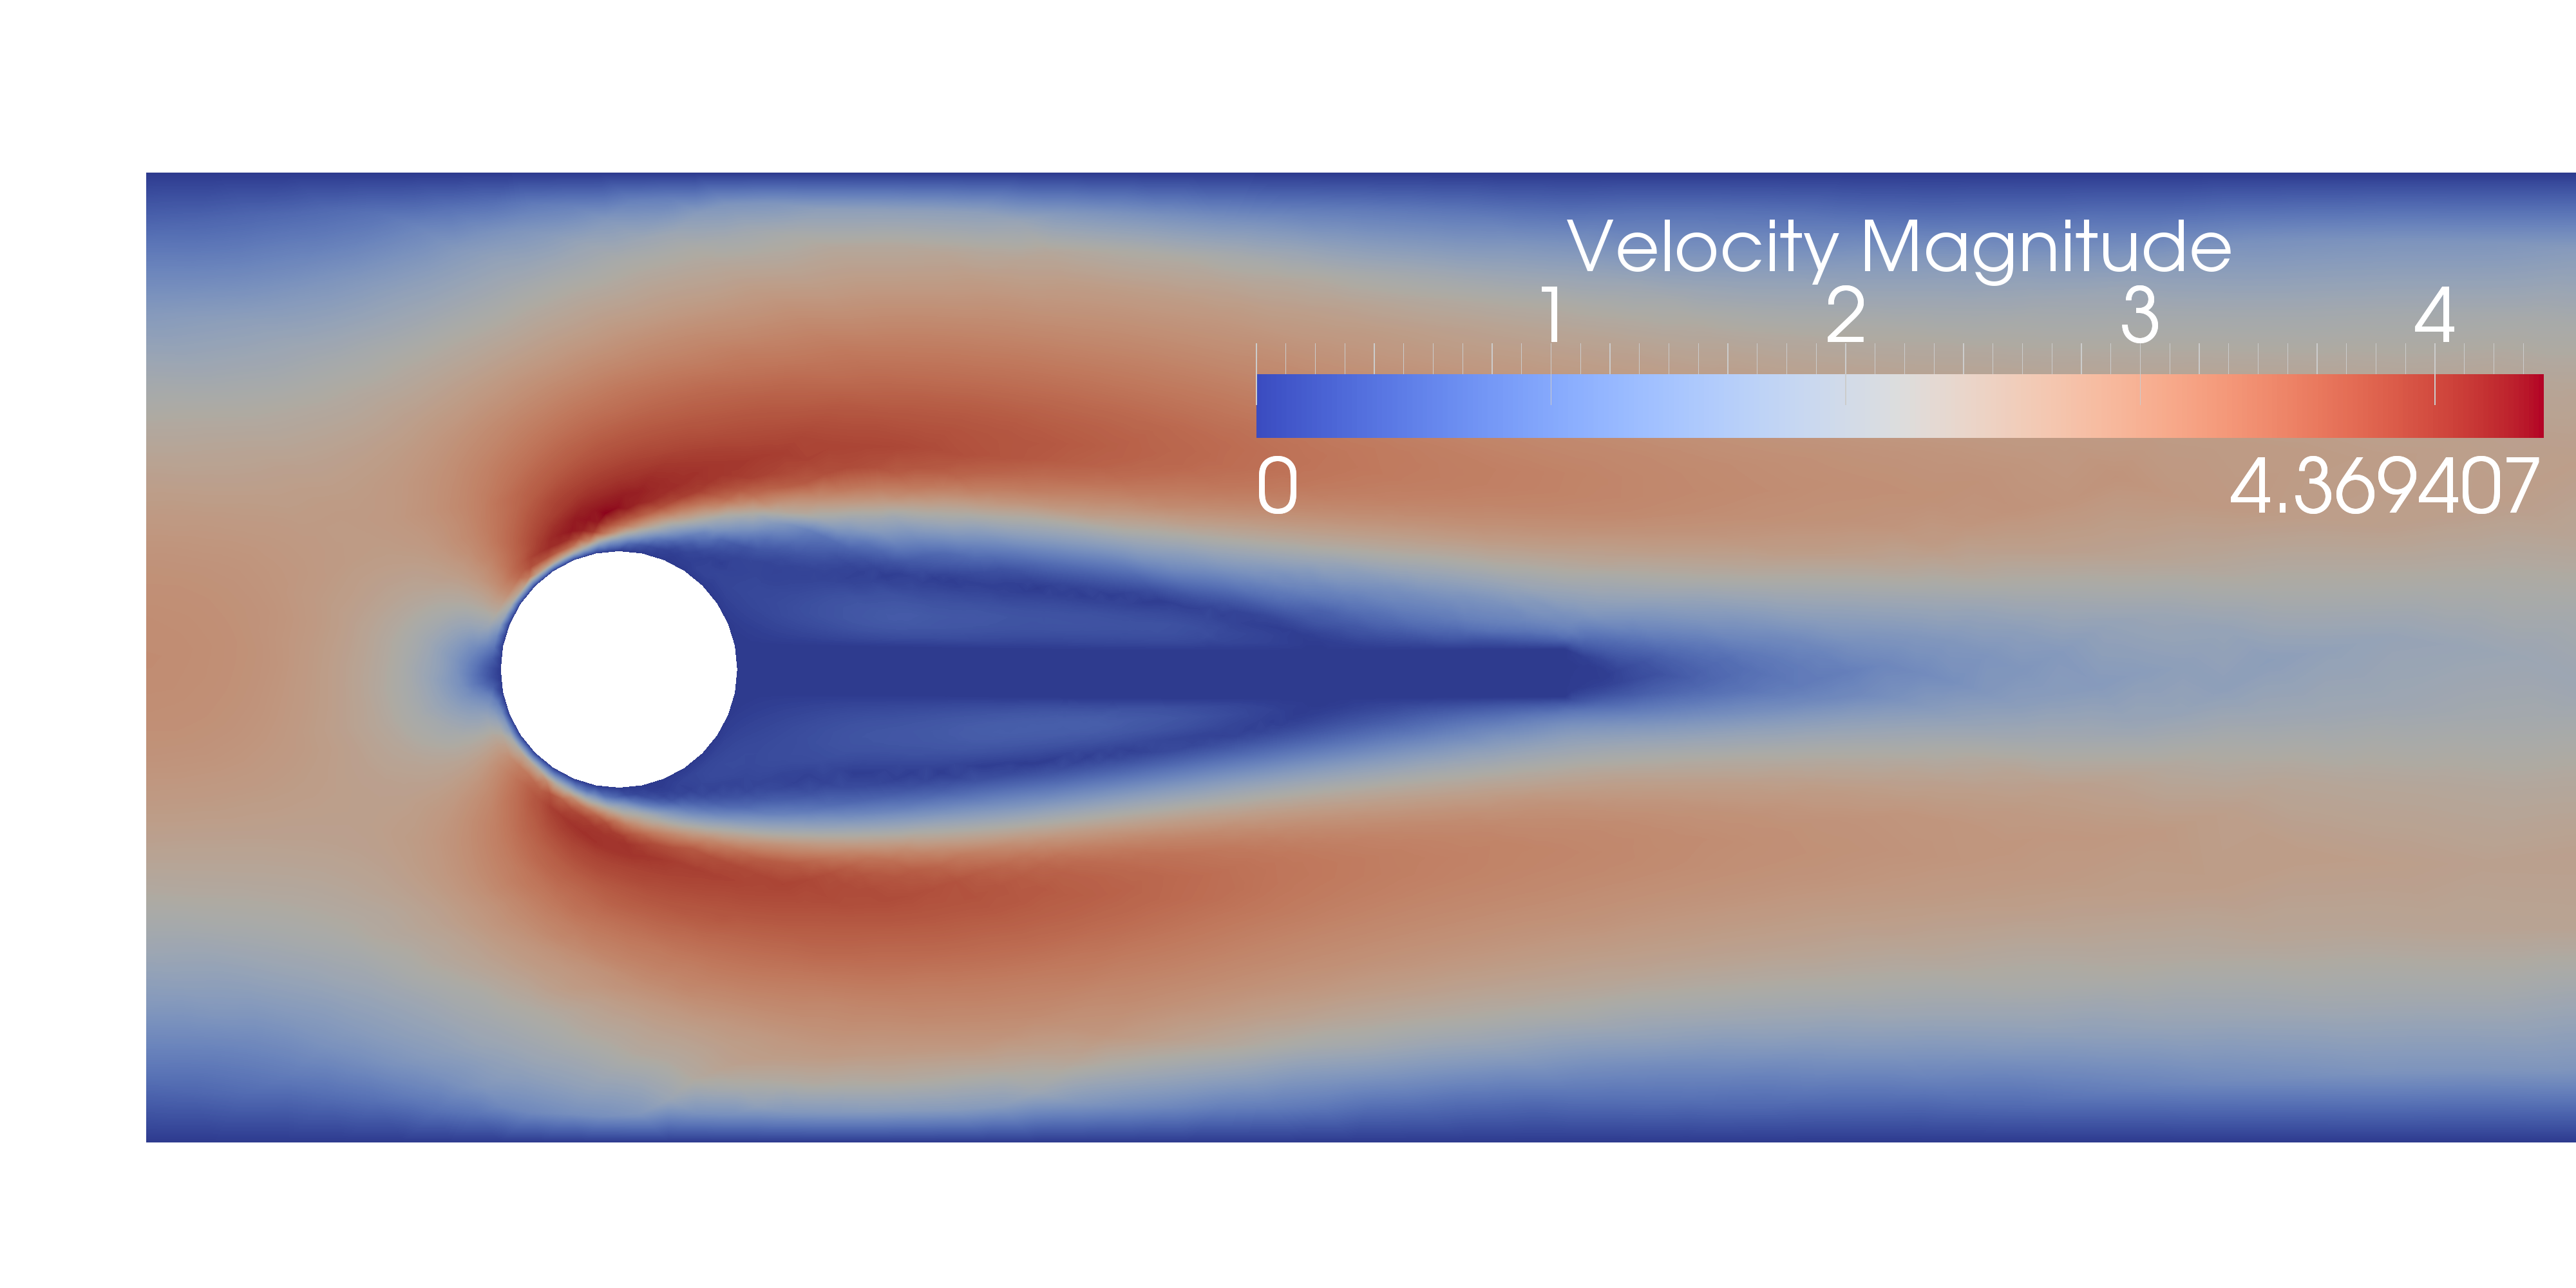
\includegraphics[width=\largefig]{chapters/hoffman-2/png/fsi3_vel_050.png}\\
  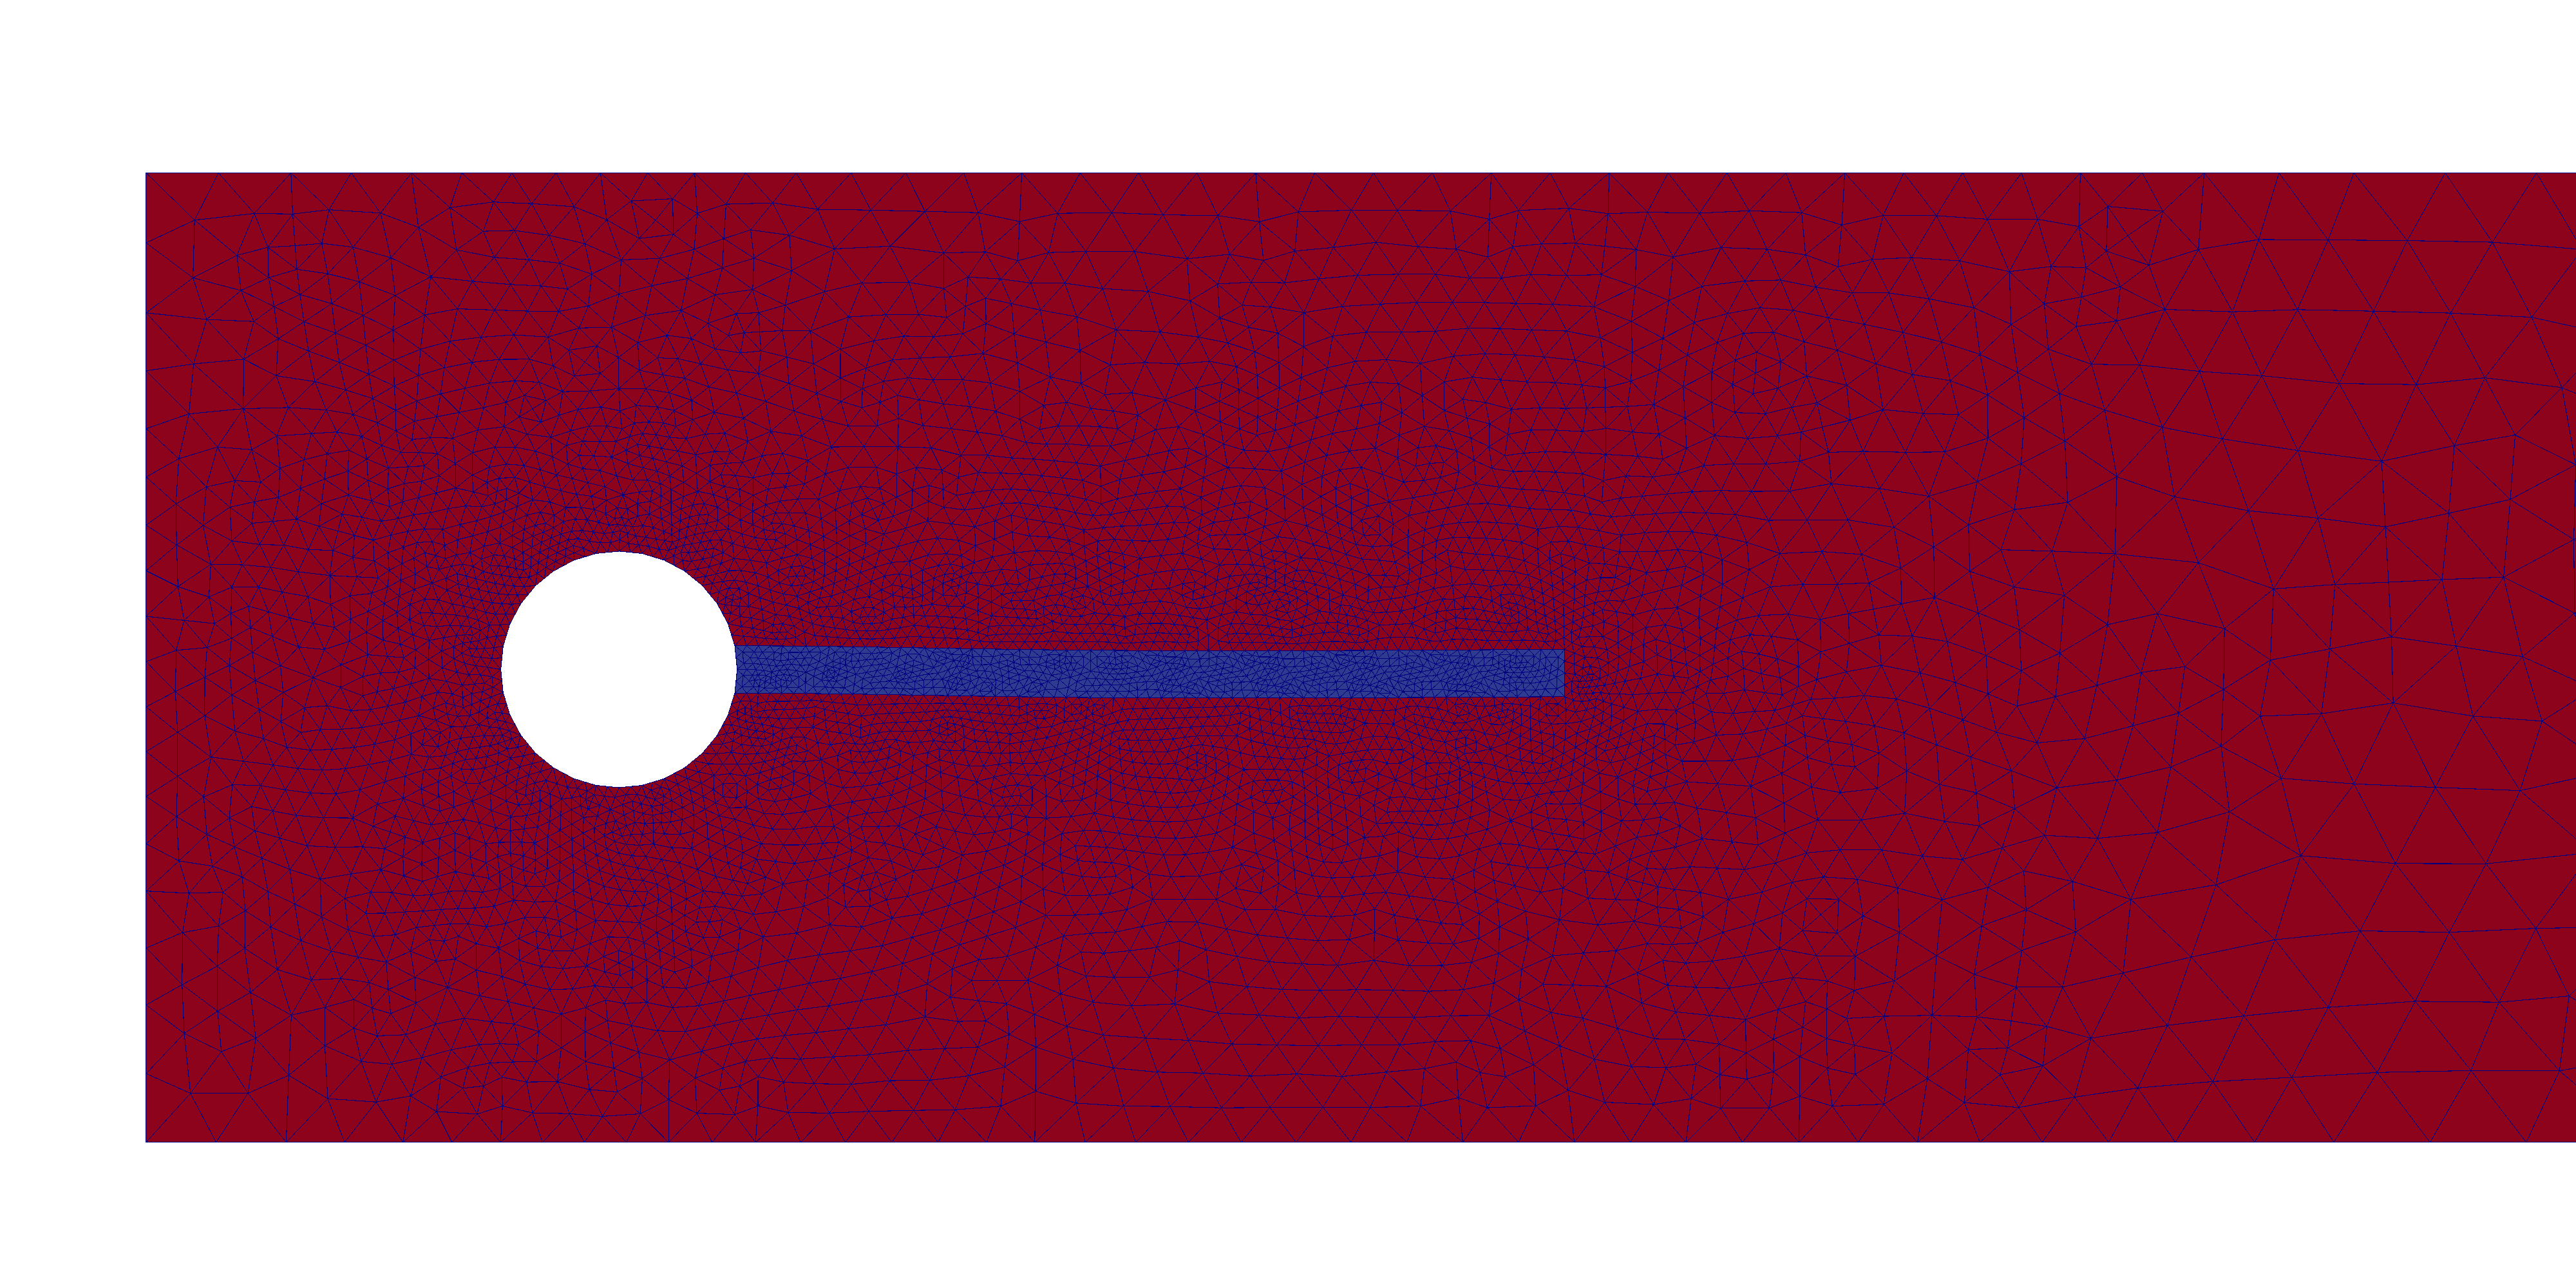
\includegraphics[width=\largefig]{chapters/hoffman-2/png/fsi3_theta_050.png}\\
  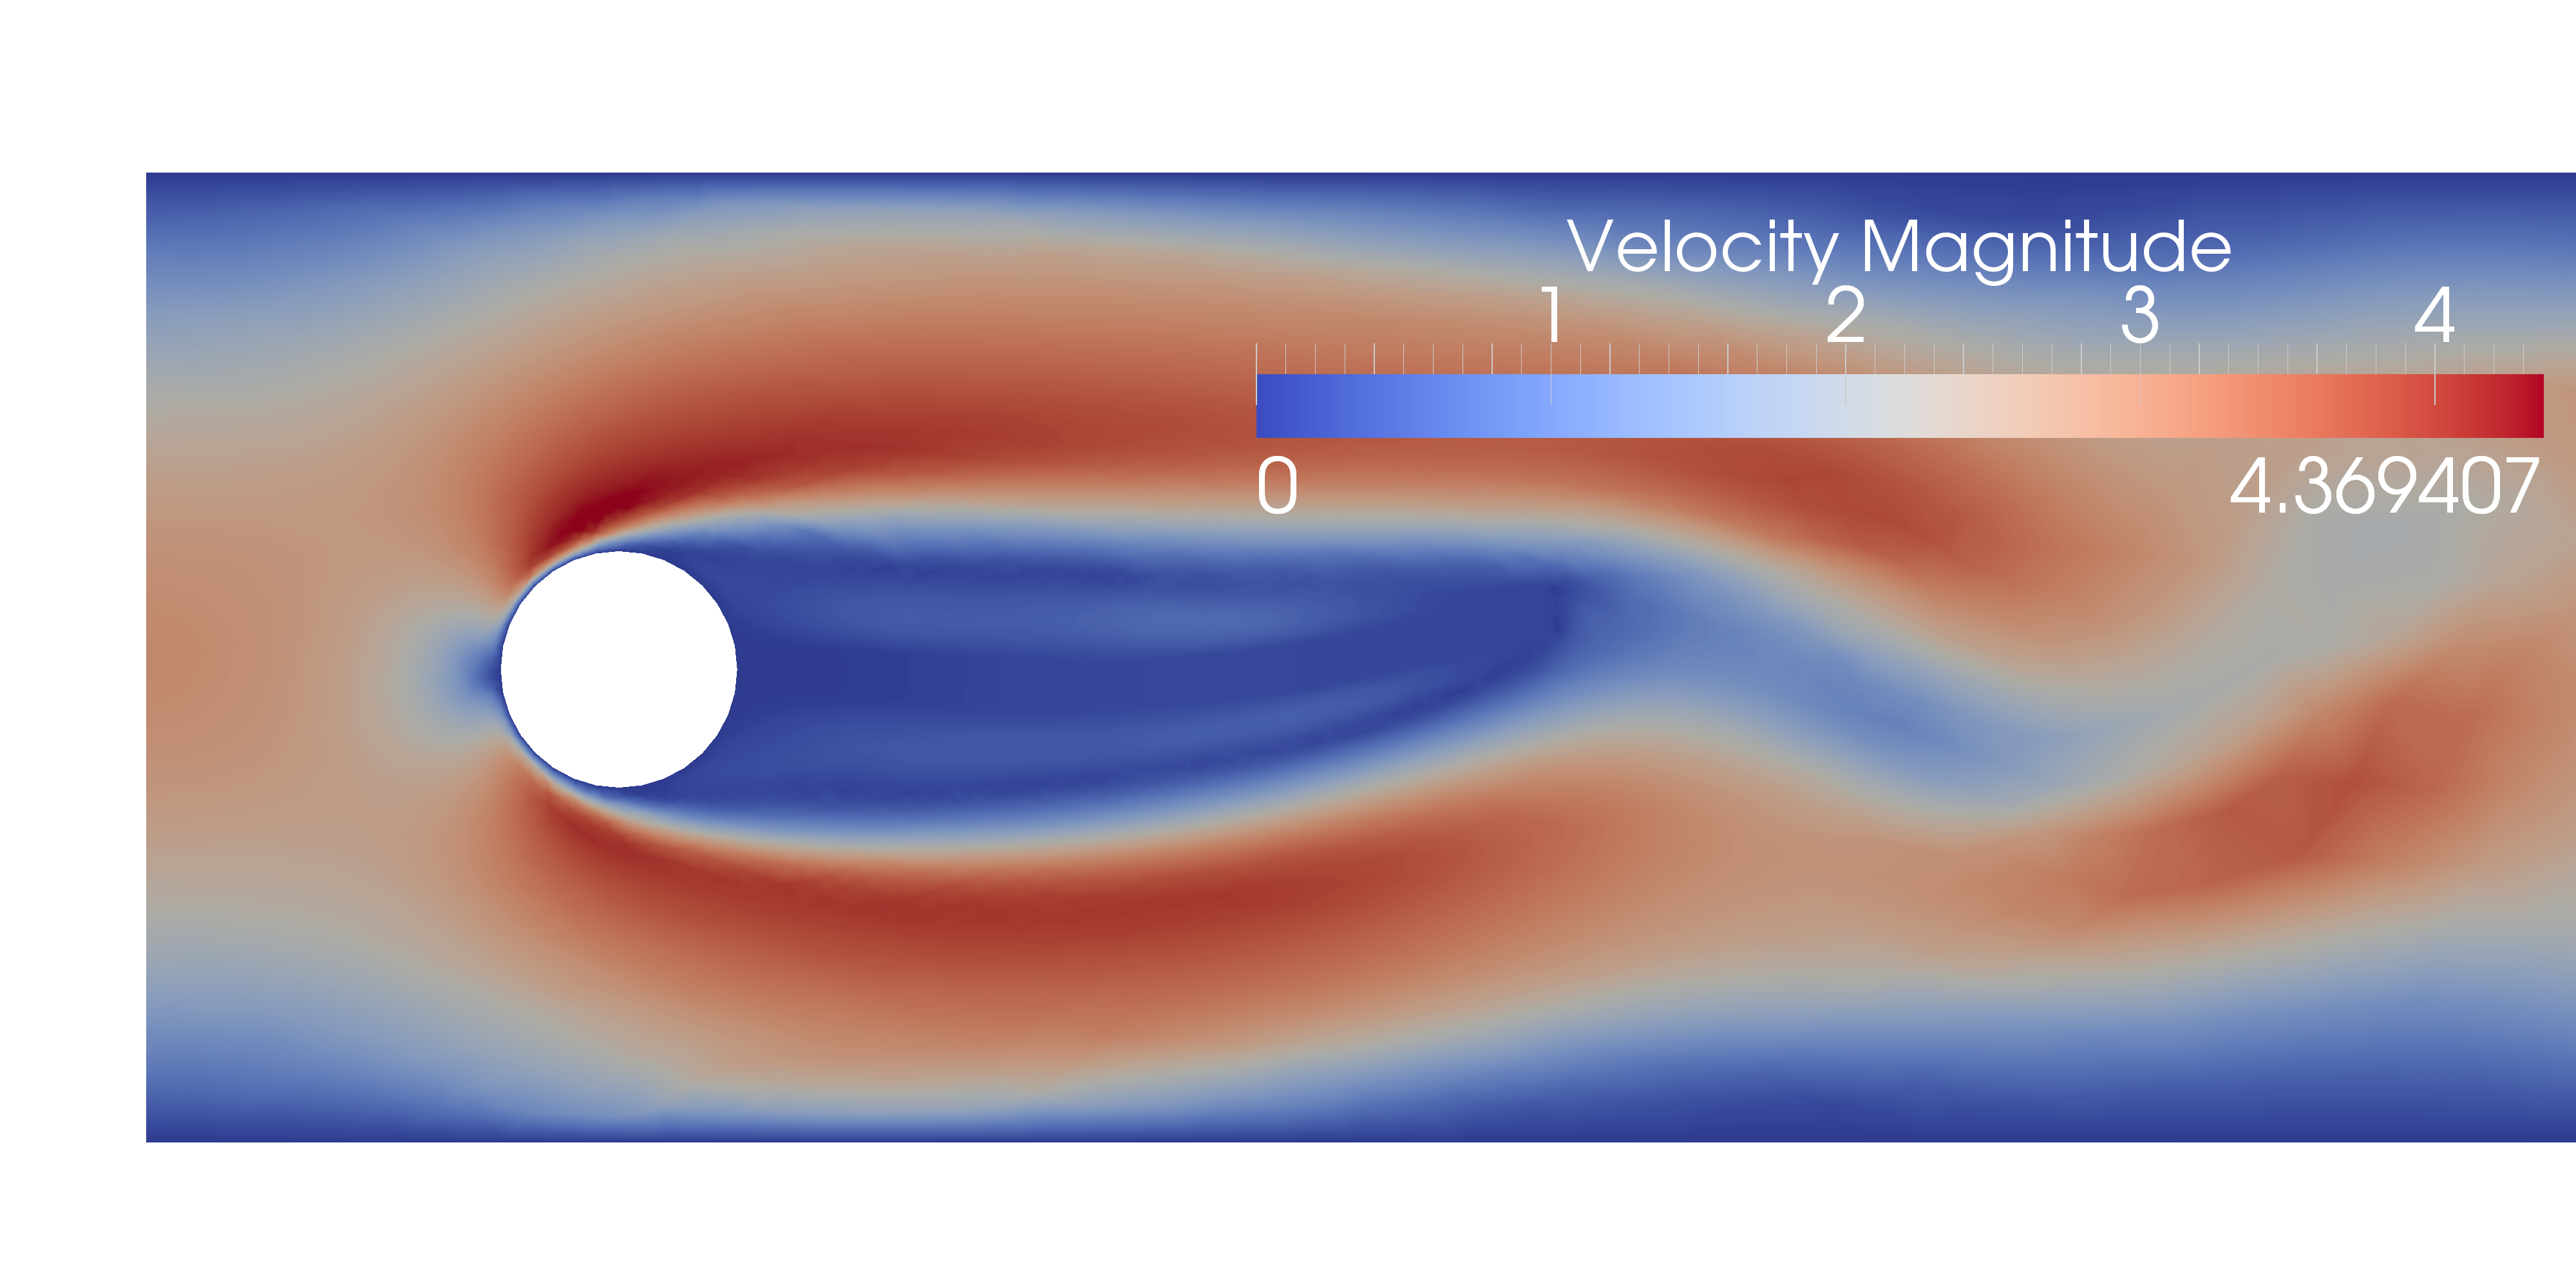
\includegraphics[width=\largefig]{chapters/hoffman-2/png/fsi3_vel_250.png}\\
  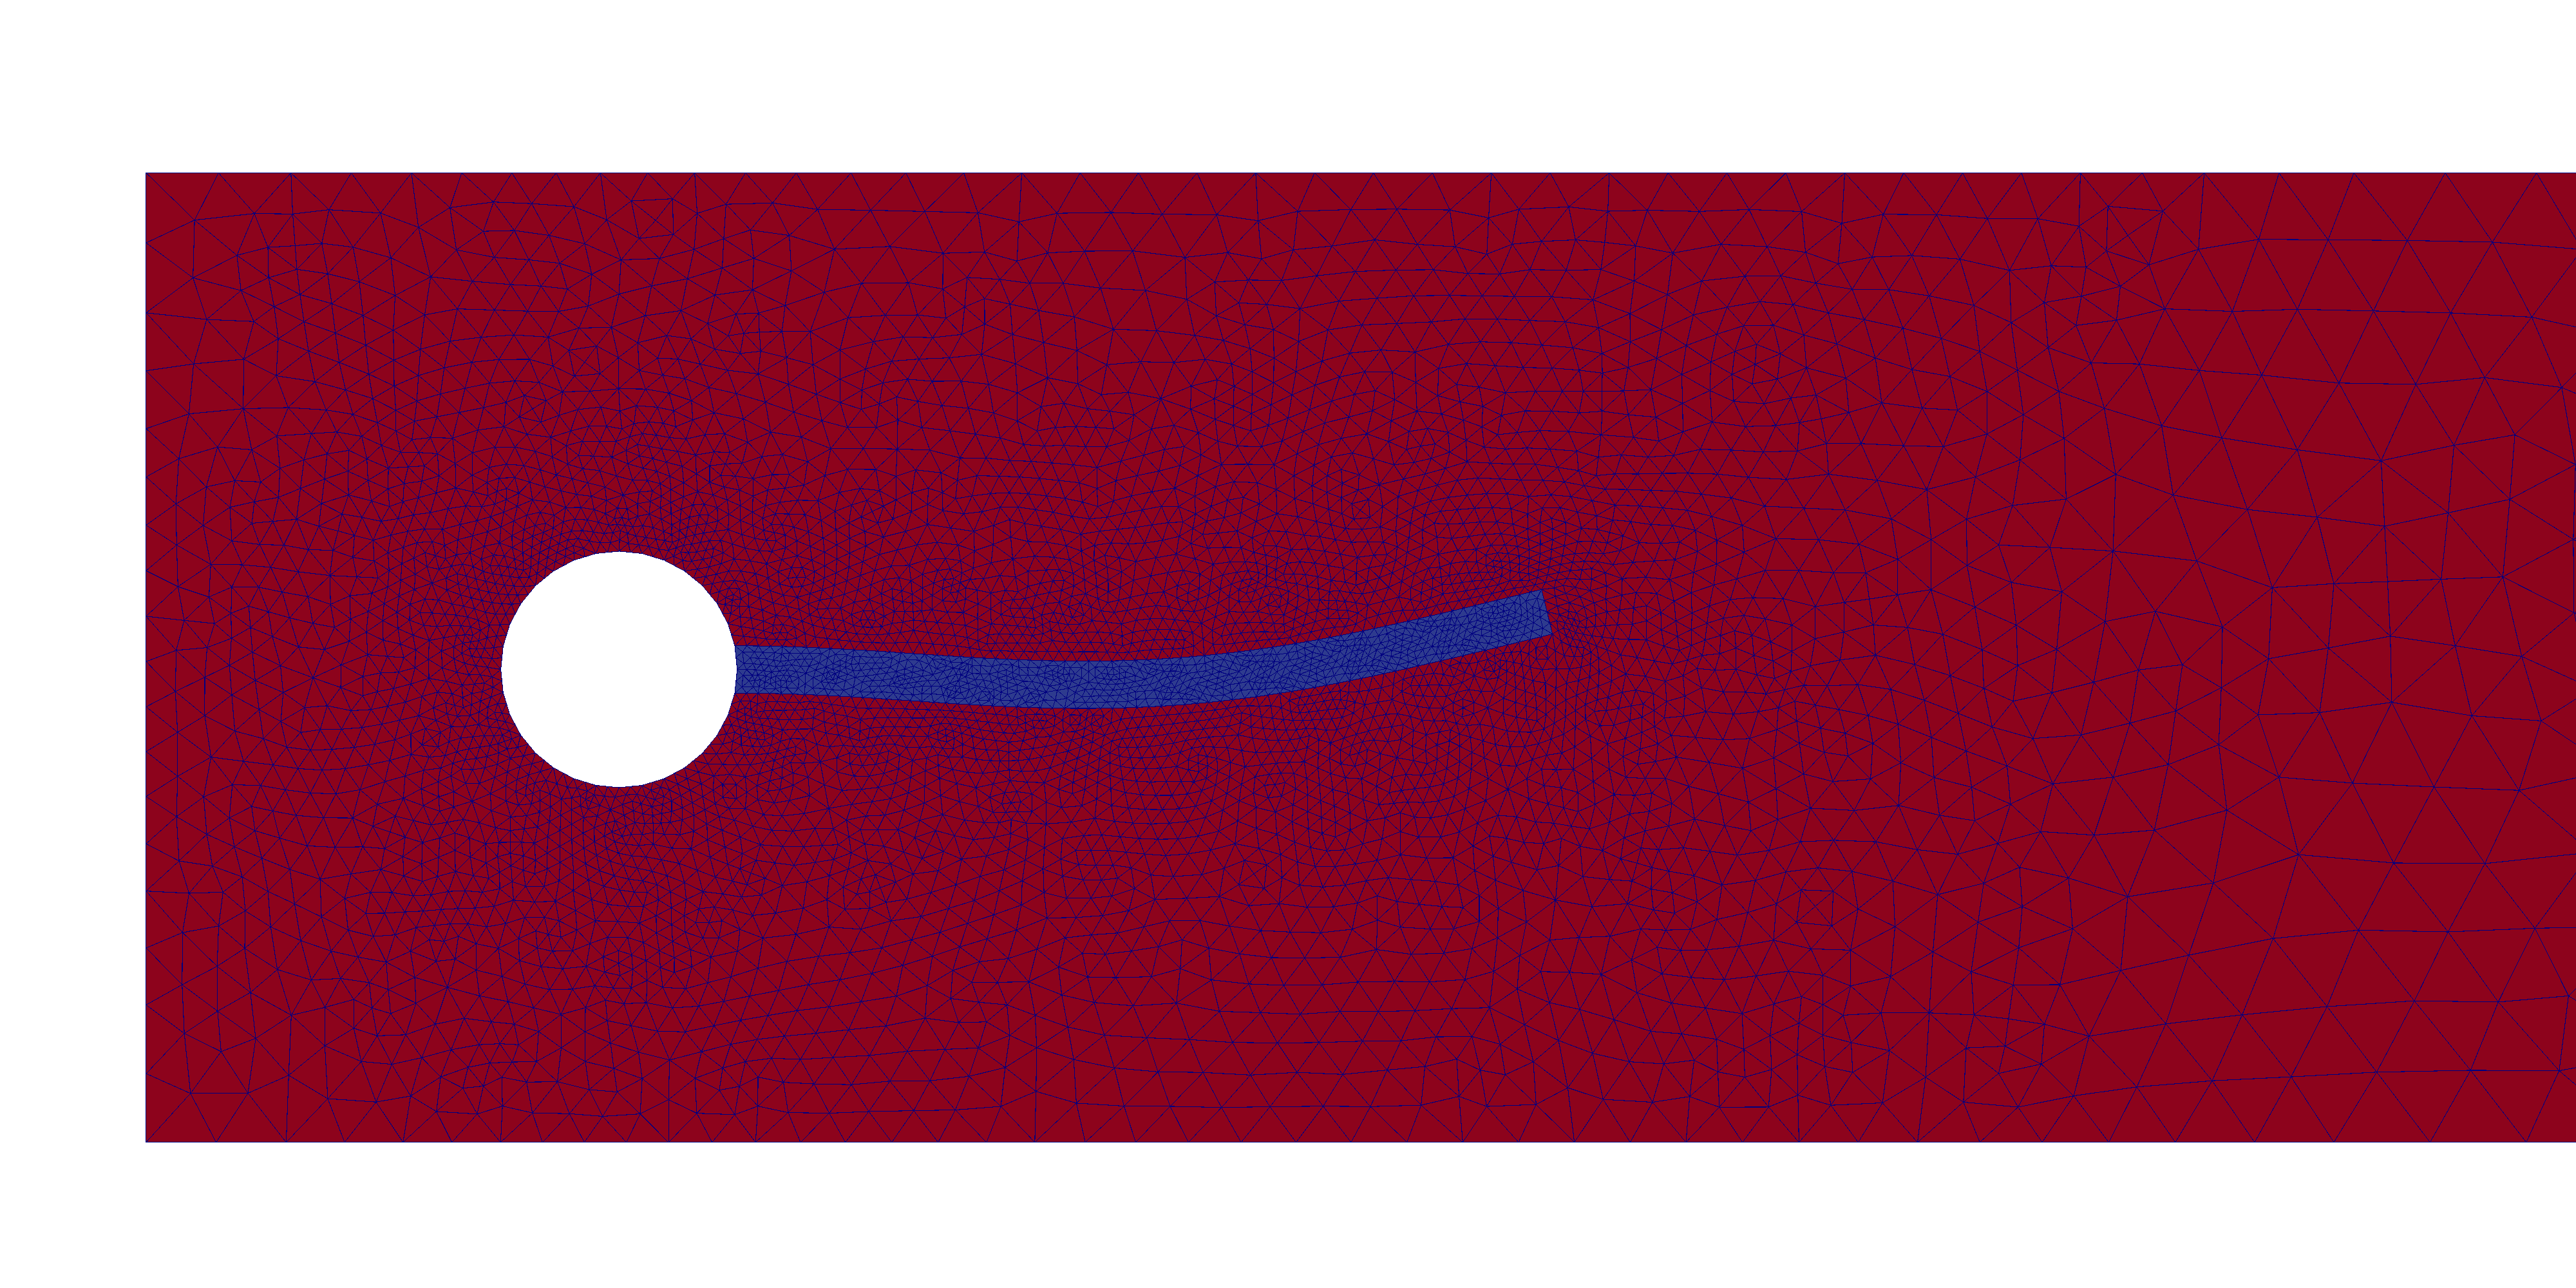
\includegraphics[width=\largefig]{chapters/hoffman-2/png/fsi3_theta_250.png}
  \caption{Velocity and phase function (with mesh) for times t = 1 and t = 5 for FSI benchmark and use case. Solution computed in parallel on a distributed meshwith 12 cores (5415 mesh points).}
  \label{fig:fsi2D_plot2}
\end{figure}

We here give a use case of solving a fluid--structure continuum
mechanics problem, where the user specifies data for modeling the
problem, and illustrates interfaces and expected outcomes. The problem
is the FLUSTRUK-A variant 3 benchmark given in \citep{HronTurek2005}
and used as verification of Unicorn
in \citep{HoffmanJanssonStockli2011} and also in
Chapter~\ref{chap:hoffman-1}. The velocity field and phase function
$\theta$ are plotted in Figure~\ref{fig:fsi2D_plot2} for times t = 1
and t = 5. We divide the use case into four parts:

\begin{description}
\item[Geometry and subdomains] \ \\ The user specifies possible
  geometrical parameters and defines subdomains. We note that for
  complex geometries the user may omit geometry information and
  specify subdomain markers as data files.
\item[Coefficients] \ \\ Known coefficients (functions appearing in the form)
  such as a force function and boundary conditions are declared.
\item[Parameters] \ \\ Simple parameters specifying material properties and numerical tolerances are given
in a parameter file.
\item[main program] \ \\ The user implements the main program and
  declares and passes data to to the solver.
\end{description}
These four parts are demonstrated by the code examples shown in
Figures~\ref{code:UseCasePart1}--\ref{code:UseCasePart4}.

\subsection{Adaptivity}

\begin{figure}
  \centering
  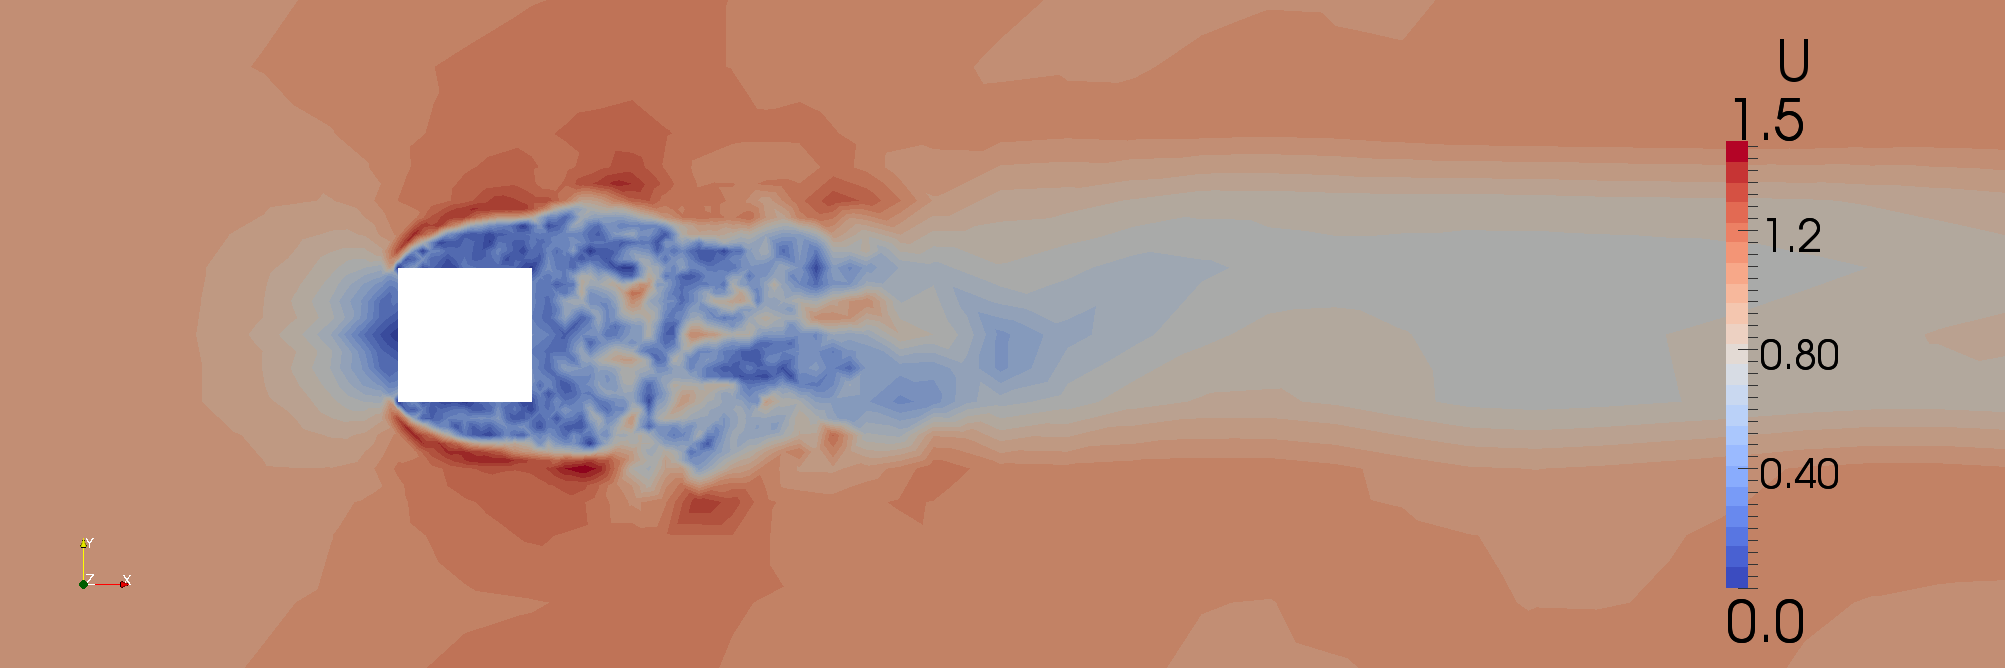
\includegraphics[width=\largefig]{chapters/hoffman-1/png/fig2b.png}
  \medskip
  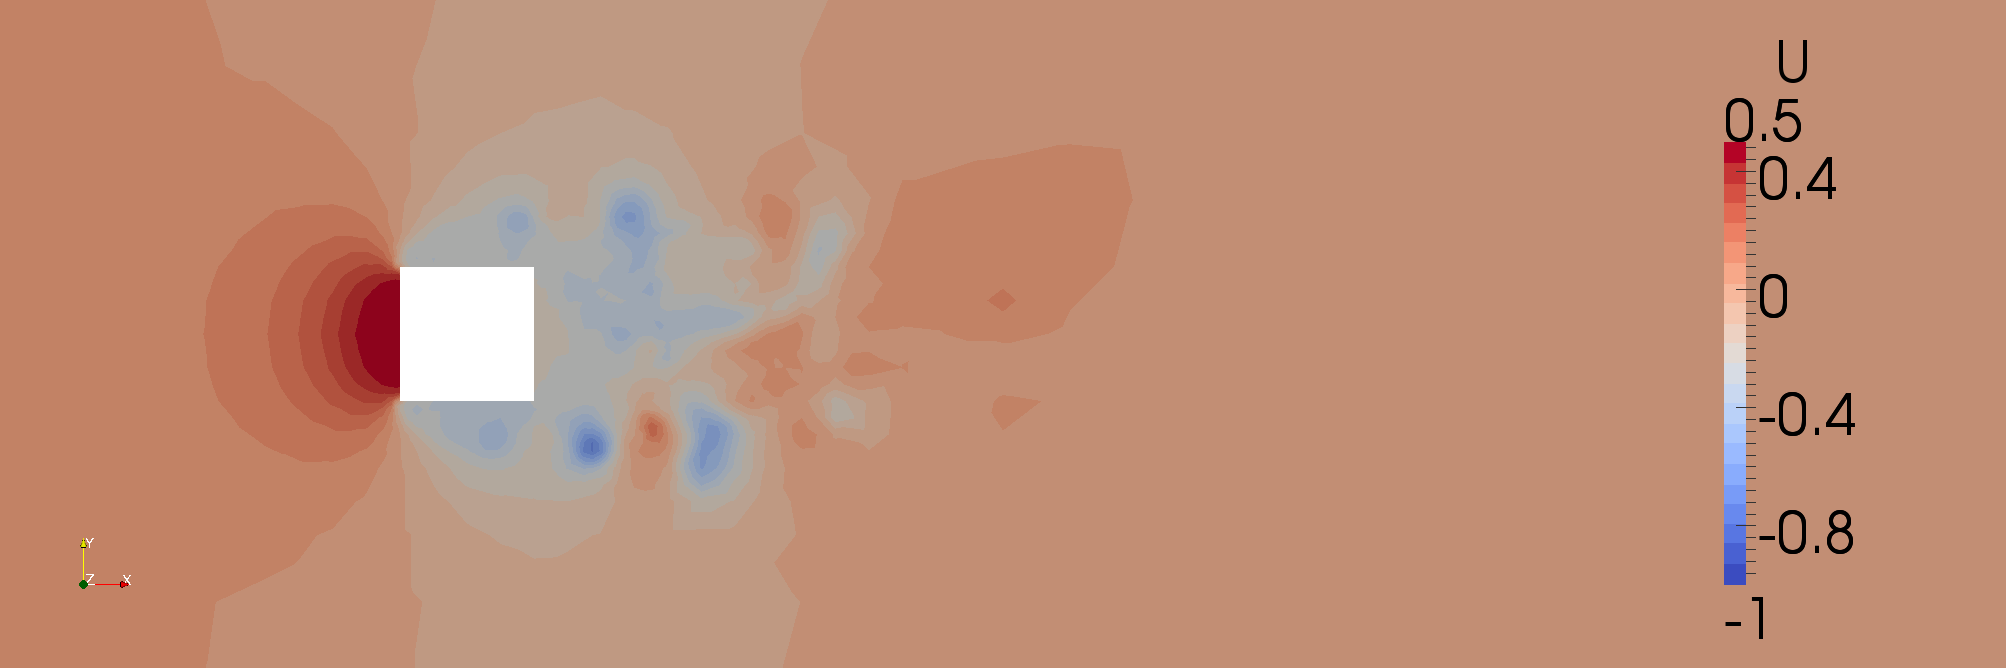
\includegraphics[width=\largefig]{chapters/hoffman-1/png/fig2c.png}
  \caption{Flow around a cube: snapshots of velocity (upper) and pressure
    (lower) for the finest mesh.}
  \label{fig:cube2}
\end{figure}

We continue with a use case for adaptive solution of a pure fluid
turbulent flow problem: flow around a 3D cube corresponding to the
cube problem description given in Chapter~\ref{chap:hoffman-1}. A
snapshot of the solution can be seen in
Figure~\ref{fig:cube2}. The implementation of the problem is
very similar to the fluid--structure case (just with pure fluid data),
but with 3 important additions:
\begin{description}
\item[Dual problem] \ \\ To compute the error estimate required by the
  adaptive algorithm, we must solve a dual problem generated by the
  primal problem and an output quantity $\psi$. Since the dual problem
  is similar in form to the primal problem, we implement both as
  variants of the same solver.

In this case we are interested in computing drag, which gives $\psi$
as a boundary condition for the dual problem:

\item[Adaptive loop] \ \\ We specify a {\tt solve()} function which computes one
  iteration of the adaptive loop: solve primal problem, solve dual
  problem, compute error estimate and check if tolerance is satisfied
  and compute adapted mesh. This function is then called in an
  adaptive loop by calling the {\tt unicorn\_solve()} function.

\begin{c++}
class Dual_BC_Momentum : public Function
{
public:
  Dual_BC_Momentum(Mesh& mesh) : Function(mesh) {}
  void eval(real* values, const real* x) const
  {
    values[0] = -1.0;
    values[1] = 0.0;
    values[2] = 0.0;
  }
};


solve()
{
  // Boundary condition for dual problem
  CubeBoundary cb;
  Dual_BC_Momentum dual_bcf_mom(mesh);

  DirichletBC dual_bc0(dual_bcf_mom, mesh, cb);

  Array <BoundaryCondition*> dual_bc_mom;
  dual_bc_mom.push_back(&dual_bc0);
  ...


  // Solve primal problem
  NSESolver primal_solver(mesh, node_normal, f, beta, aero_f, primal_bc_mom, primal_bc_con,
    chkp, w_limit, td, ``primal'');
  primal_solver.solve();

  // Solve dual problem (gives weight for error estimate)
  NSESolver dual_solver(mesh, node_normal, f, beta, aero_f, dual_bc_mom, dual_bc_con,
    chkp, w_limit, td, ``dual'');
  dual_solver.solve();
}

\end{c++}

\item[Slip boundary condition] \ \\ For turbulent flow, we model the
  boundary layer as a friction boundary condition. We specify the
  normal component as a strong slip boundary condition used just as a
  regular Dirichlet boundary condition.
%%
\begin{c++}
NodeNormal node_normal(mesh);
SlipBoundary sb;

SlipBC slip_bc(mesh, sb, node_normal);

Array <BoundaryCondition*> primal_bc_mom;
primal_bc_mom.push_back(&slip_bc);
\end{c++}

\end{description}

\begin{figure}
\begin{c++}
#include <dolfin.h>
#include <unicorn/UCSolver.h>

using namespace dolfin;
using namespace dolfin::unicorn;

real bmarg = 1.0e-6 + DOLFIN_EPS;

namespace Geo
{
  // Geometry details
  real box_L = 2.5;
  real box_H = 0.41;

  real xmin = 0.0; real xmax = box_L;
  real ymin = 0.0; real ymax = box_H;
}

// Sub domain for inflow
class InflowBoundary : public SubDomain
{
public:
  bool inside(const real* p, bool on_boundary) const
  {
    return on_boundary && (p[0] < Geo::xmax - bmarg ||
                           p[1] < Geo::ymin + bmarg ||
                           p[1] > Geo::ymax - bmarg);
  }
};

// Sub domain for outflow
class OutflowBoundary : public SubDomain
{
public:
  bool inside(const real* p, bool on_boundary) const
  {
    InflowBoundary ib;

    return on_boundary && !ib.inside(p, on_boundary);
  }
};
\end{c++}
\caption{Part 1 of Unicorn solver FSI use case: geometry and subdomains.}
\label{code:UseCasePart1}
\end{figure}

\begin{figure}
\begin{c++}
// Force term
class ForceFunction : public Function
{
public:
  ForceFunction(Mesh& mesh, TimeDependent& td) :
    Function(mesh), td(td) {}
  void eval(real* values, const real* x) const
  {
    int d = cell().dim();

    for (int i = 0; i < d; i++)
    {
      values[i] = 0.0;
    }
  }

  TimeDependent& td;
};

// Boundary condition for momentum equation
class BC_Momentum : public Function
{
public:
  BC_Momentum(Mesh& mesh) :
    Function(mesh) {}
  void eval(real* values, const real* x) const
  {
    int d = cell().dim();

    for (int i = 0; i < d; i++)
    {
      values[i] = 0.0;
    }
    if (x[0] < (Geo::xmin + bmarg))
    {
      // Define a parabolic inflow profile
      real Um = 2.0;
      values[0] =
        ramp*1.5*Um*( (x[1]*(Geo::cont_H - x[1])) /
          ((0.5*Geo::cont_H)*(0.5*Geo::cont_H)) );
  }
};

// Initial condition for phase variable
class BisectionFunction : public Function
{
public:
  BisectionFunction(Mesh& mesh) : Function(mesh) {}
  void eval(real* values, const real* p) const
  {
    bool condition =
      (((flag_start_x - bmarg) < p[0] &&
         p[0] < (flag_end_x + bmarg)) &&
       ((flag_start_y - bmarg) < p[1] &&
         p[1] < (flag_end_y + bmarg)));

    if(condition)
      values[0] = 0.0;
    else
      values[0] = 1.0;
  }
};
\end{c++}
\caption{Part 2 of Unicorn solver FSI use case: coefficients.}
\label{code:UseCasePart2}
\end{figure}

\begin{figure}
\begin{c++}
Parameters for Unicorn solver:

0.0       beta - friction coefficient
0.001     nu - viscosity
2.0e3     mu - solid stiffness
0.0e0     nu_s - solid damping
1.0e0     rho_s - solid density

10        n_samples - number of samples
1         adapt_iter - number of adaptive iterations
0.001     adapt_tol - adaptive tolerance
10        adapt_percentage - adaptive percentage
rivara    adapt_algorithm - adaptive refinement type

10.0       T - final time, primal solver
0.25      dual_T - final time, dual solver
1.0       Ubar - free stream velocity

gmres     krylov_method - krylov method
amg       krylov_pc - preconditioner
\end{c++}
\caption{Part 3 of FSI use case: parameter file}
\label{code:UseCasePart3}
\end{figure}

\begin{figure}
\begin{c++}
void solve(Mesh& mesh, Checkpoint& chkp,
  long& w_limit, timeval& s_time)
{
  InflowBoundary iboundary;
  BC_Momentum bcf_mom(mesh);
  ForceFunction f(mesh);

  DirichletBC bc_mom0(bcf_mom, mesh, iboundary);

  Array <BoundaryCondition*> bc_mom;
  bc_mom.push_back(&bc_mom0);

  Array<Function*> aero_f;

  ...

  NSESolver psolver(mesh, node_normal, f, beta, aero_f, bc_mom, bc_con,
    chkp, w_limit, td, ``primal'');
  psolver.solve();
}

int main()
{
  Mesh mesh;
  ...

  unicorn_init(argc, argv, mesh, chkp, w_limit, iter);

  unicorn_solve(mesh, chkp, w_limit, s_time, iter, 0, 0, &solve);
  return 0;
}
\end{c++}
\caption{Part 4 of FSI use case: structure of main program, passing data to solver.}
\label{code:UseCasePart4}
\end{figure}

\subsection{Unicorn-HPC installation and basic test}

Unicorn-HPC is the high-performance computing branch of Unicorn,
showing strong linear scaling on massively parallel hardware as
described above.

To verify the correct installation and functionality of Unicorn-HPC,
follow the steps in the README file in the Unicorn-HPC distribution,
under ``Testing''. The test represents the turbulent flow past a cube
simulation described in Chapter~\ref{chap:hoffman-1} and above.

%------------------------------------------------------------------------------
\section{Acknowledgments}

We acknowledge contributions to Unicorn, both software development as
well as ideas and scientific support from: Mattias Aechtner, Peter
Brune, Zilan Ciftci, G\"aetan Compere, Claes Johnson, Ashraful Kadir,
Jeannette Sp\"uhler, Michael St\"ockli and Rodrigo Vilela de Abreu.
